%
% Copyright 2018 Joel Feldman, Andrew Rechnitzer and Elyse Yeager.
% This work is licensed under a Creative Commons Attribution-NonCommercial-ShareAlike 4.0 International License.
% https://creativecommons.org/licenses/by-nc-sa/4.0/
%
\questionheader{ex:s1.1}

%%%%%%%%%%%%%%%%%%
\subsection*{\Conceptual}
%%%%%%%%%%%%%%%%%%

\Instructions{For Questions~\ref{concept_int_a} through \ref{concept_int_b}, we want you to develop an understanding of the model we are using to define an integral: we approximate the area under a curve by bounding it between rectangles. Later, we will learn more sophisticated methods of integration, but they are all based on this simple concept.}
\begin{question}\label{concept_int_a}
Give a range of possible values for the shaded area in the picture below.
\begin{center}
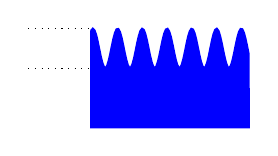
\begin{tikzpicture}
\YEaaxis{1}{4}{1}{2}
\draw[thick, blue, fill] plot[domain=1:3, samples=100] (\x,{.25*sin(20*\x r)+1})--(3,0)--(1,0)--(1,1.23);
\YExcoord{1}{1};
\YExcoord{3}{3};
\YEycoord{0.75}{0.75};
\YEycoord{1.25}{1.25};
\foreach \x in {0.75,1.25}{\draw[dotted] (.2,\x)--(1,\x);}
\end{tikzpicture}
\end{center}
\end{question}
\begin{hint}
Draw a rectangle that \emph{encompasses} the entire shaded area, and one that is \emph{encompassed by} the shaded area. The shaded area is no more than the area of the bigger rectangle, and no less than the area of the smaller rectangle.
\end{hint}
\begin{answer}
The area is between $1.5$ and $2.5$ square units.
\end{answer}
\begin{solution}
\begin{center}
\begin{tikzpicture}
\YEaaxis{1}{4}{1}{2}
\draw[thick, blue, fill] plot[domain=1:3, samples=100] (\x,{.25*sin(20*\x r)+1})--(3,0)--(1,0)--(1,1.23);
\YExcoord{1}{1};
\YExcoord{3}{3};
\YEycoord{0.75}{0.75};
\YEycoord{1.25}{1.25};
\foreach \x in {0.75,1.25}{\draw[dotted] (.2,\x)--(1,\x);}
\draw[red, pattern=crosshatch, pattern color=red] (1,1.25)--(3,1.25)--(3,0)--(1,0)--cycle;
\end{tikzpicture}
\qquad
\begin{tikzpicture}
\YEaaxis{1}{4}{1}{2}
\draw[thick, blue, fill] plot[domain=1:3, samples=100] (\x,{.25*sin(20*\x r)+1})--(3,0)--(1,0)--(1,1.23);
\YExcoord{1}{1};
\YExcoord{3}{3};
\YEycoord{0.75}{0.75};
\YEycoord{1.25}{1.25};
\foreach \x in {0.75,1.25}{\draw[dotted] (.2,\x)--(1,\x);}
\draw[red, pattern=crosshatch, pattern color=red] (1,0.75)--(3,0.75)--(3,0)--(1,0)--cycle;
\end{tikzpicture}
\end{center}
The diagram on the left shows a rectangle with area $2 \times 1.25=2.5$ square  units. Since the blue-shaded region is entirely inside this rectangle, the area of the blue-shaded region is no more than 2.5 square units.

The diagram on the right shows a rectangle with area $2 \times 0.75=1.5$ square  units. Since the blue-shaded region contains this entire rectangle, the area of the blue region is no less than 1.5 square units.

So, the area of the blue-shaded region is between 1.5 and 2.5 square units.

Remark: we could also give an obvious range, like ``the shaded area is between zero and one million square units." This would be true, but not very useful or interesting.
\end{solution}


\begin{Mquestion}
Give a range of possible values for the shaded area in the picture below.
\begin{center}
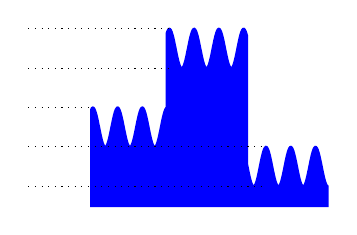
\begin{tikzpicture}
\YEaaxis{1.5}{5}{1}{3}
\draw[thick, blue, fill] plot[domain=1:1.96, samples=100] (\x,{.25*sin(20*\x r)+1})--
plot[domain=1.96:2.98, samples=100] (\x,{.25*sin(20*(\x-1.6) r )+2})--
plot[domain=2.98:4, samples=100] (\x,{.25*sin(20*\x r)+.5})--(4,0)--(1,0)--(1,1.23);
\YExcoord{1}{1};
\YExcoord{1.96}{2};
\YExcoord{2.98}{3};
\YExcoord{4}{4};

\YEycoord{0.75}{0.75};
\YEycoord{1.25}{1.25};
\YEycoord{0.25}{0.25};
\YEycoord{2.25}{2.25};
\YEycoord{1.75}{1.75};

\foreach \x in {0.75, 0.25}{\draw[dotted] (.2,\x)--(3.2,\x);}
\foreach \x in {1.75,2.25}{\draw[dotted] (.2,\x)--(2,\x);}
\foreach \x in {1.25}{\draw[dotted] (.2,\x)--(1,\x);}

\end{tikzpicture}
\end{center}
\end{Mquestion}
\begin{hint}
We can improve on the method of Question~\ref{concept_int_a} by using three rectangles that together encompass the shaded region, and three rectangles that together are encompassed by the shaded region.
\end{hint}
\begin{answer}
The shaded area is between 2.75 and 4.25 square units. (Other estimates are possible, but this is a reasonable estimate, using methods from this chapter.)
\end{answer}
\begin{solution}

\begin{description}
\item[Solution 1:]
One naive way to solve this is to simply use the same method as Question~\ref{concept_int_a}.

\begin{center}
\begin{tikzpicture}
\YEaaxis{1.5}{5}{1}{3}
\draw[thick, blue, fill] plot[domain=1:1.96, samples=100] (\x,{.25*sin(20*\x r)+1})--
plot[domain=1.96:2.98, samples=100] (\x,{.25*sin(20*(\x-1.6) r )+2})--
plot[domain=2.98:4, samples=100] (\x,{.25*sin(20*\x r)+.5})--(4,0)--(1,0)--(1,1.23);
\YExcoord{1}{1};
\YExcoord{1.96}{2};
\YExcoord{2.98}{3};
\YExcoord{4}{4};

\YEycoord{0.75}{0.75};
\YEycoord{1.25}{1.25};
\YEycoord{0.25}{0.25};
\YEycoord{2.25}{2.25};
\YEycoord{1.75}{1.75};
\draw[dotted] (.2,2.25)--(1,2.25);
\draw[red, pattern=crosshatch, pattern color=red] (1,2.25)--(4,2.25)--(4,0)--(1,0)--cycle;
\end{tikzpicture}
\qquad
\begin{tikzpicture}
\YEaaxis{1.5}{5}{1}{3}
\draw[thick, blue, fill] plot[domain=1:1.96, samples=100] (\x,{.25*sin(20*\x r)+1})--
plot[domain=1.96:2.98, samples=100] (\x,{.25*sin(20*(\x-1.6) r )+2})--
plot[domain=2.98:4, samples=100] (\x,{.25*sin(20*\x r)+.5})--(4,0)--(1,0)--(1,1.23);
\YExcoord{1}{1};
\YExcoord{1.96}{2};
\YExcoord{2.98}{3};
\YExcoord{4}{4};

\YEycoord{0.75}{0.75};
\YEycoord{1.25}{1.25};
\YEycoord{0.25}{0.25};
\YEycoord{2.25}{2.25};
\YEycoord{1.75}{1.75};
\draw[dotted] (.2,.25)--(1,.25);
\draw[red, pattern=crosshatch, pattern color=red] (1,0.25)--(4,0.25)--(4,0)--(1,0)--cycle;
\end{tikzpicture}
\end{center}
 The rectangle on the left has area $3 \times 2.25 = 6.75$ square units, and encompasses the entire shaded region.
  The rectangle on the right has area $3 \times 0.25 = 0.75$ square units, and is entirely contained inside the blue-shaded region. So, the area of the blue-shaded region is between 0.75 and 6.75 square units.

 This is a legitimate approximation, but we can easily do much better. The shape of this graph suggests that using the areas of \emph{three} rectangles would be a natural way to improve our estimate.
 \item[Solution 2:]
Let's use these rectangles instead:
\begin{center}
\begin{tikzpicture}
\YEaaxis{1}{5}{1}{3}
\draw[thick, blue, fill] plot[domain=1:1.96, samples=100] (\x,{.25*sin(20*\x r)+1})--
plot[domain=1.96:2.98, samples=100] (\x,{.25*sin(20*(\x-1.6) r )+2})--
plot[domain=2.98:4, samples=100] (\x,{.25*sin(20*\x r)+.5})--(4,0)--(1,0)--(1,1.23);
\YExcoord{1}{1};
\YExcoord{1.96}{2};
\YExcoord{2.98}{3};
\YExcoord{4}{4};

\YEycoord{0.75}{0.75};
\YEycoord{1.25}{1.25};
\YEycoord{0.25}{0.25};
\YEycoord{2.25}{2.25};
\YEycoord{1.75}{1.75};

\foreach \x in {0.75, 0.25}{\draw[dotted] (.2,\x)--(3.2,\x);}
\foreach \x in {1.75,2.25}{\draw[dotted] (.2,\x)--(2,\x);}
\foreach \x in {1.25}{\draw[dotted] (.2,\x)--(1,\x);}


\draw[red, pattern=crosshatch, pattern color=red] (1,1.25)-| (2,2.25)-|(3,0.75)-|(4,0)--(1,0)--cycle;
\end{tikzpicture}
\qquad
\begin{tikzpicture}
\YEaaxis{1}{5}{1}{3}
\draw[thick, blue, fill] plot[domain=1:1.96, samples=100] (\x,{.25*sin(20*\x r)+1})--
plot[domain=1.96:2.98, samples=100] (\x,{.25*sin(20*(\x-1.6) r )+2})--
plot[domain=2.98:4, samples=100] (\x,{.25*sin(20*\x r)+.5})--(4,0)--(1,0)--(1,1.23);
\YExcoord{1}{1};
\YExcoord{1.96}{2};
\YExcoord{2.98}{3};
\YExcoord{4}{4};

\YEycoord{0.75}{0.75};
\YEycoord{1.25}{1.25};
\YEycoord{0.25}{0.25};
\YEycoord{2.25}{2.25};
\YEycoord{1.75}{1.75};

\foreach \x in {0.75, 0.25}{\draw[dotted] (.2,\x)--(3.2,\x);}
\foreach \x in {1.75,2.25}{\draw[dotted] (.2,\x)--(2,\x);}
\foreach \x in {1.25}{\draw[dotted] (.2,\x)--(1,\x);}


\draw[red, pattern=crosshatch, pattern color=red] (1,0.75)-| (2,1.75)-|(3,0.25)-|(4,0)--(1,0)--cycle;
\end{tikzpicture}
\end{center}
In the left picture, the red area is $(1 \times 1.25)+(1 \times 2.25)+(1 \times 0.75)=4.25$ square units. In the right picture, the red area is $(1 \times 0.75)+(1 \times 1.75)+(1 \times 0.25)=2.75$ square units. So, the blue shaded area is between 2.75 and 4.25 square units.
 \end{description}
\end{solution}

\begin{question}
Using rectangles, find a lower and upper bound for $\displaystyle\int_1^3 \dfrac{1}{2^x}\dee{x}$ that differ by at most 0.2 square units.
\begin{center}
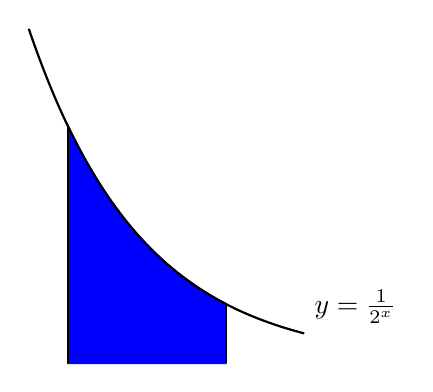
\begin{tikzpicture}
\YEaaxis{1}{5}{1}{5}
\draw[thick, blue, fill] plot[domain=1:3, samples=100] (\x,{6*pow(.5,\x)})--(3,0)--(1,0)--cycle;
\draw[thick] plot[domain=0.5:4, samples=100] (\x,{6*pow(.5,\x)}) node[above right]{$y=\frac{1}{2^x}$};
\YExcoord{1}{1};
\YExcoord{3}{3};
\draw[thick] (1,0)--(1,3) (3,0)--(3,.75);
\end{tikzpicture}
\end{center}
\end{question}
\begin{hint}
Four rectangles suffice.
\end{hint}
\begin{answer}
The area under the curve is a number in the interval $\left( \frac{3}{8}\left[\frac{1}{2}+\frac{1}{\sqrt{2}}\right], \frac{3}{8}\left[1+\frac{1}{\sqrt{2}}\right]\right)$.
\end{answer}
\begin{solution}
Remark: in the solution below, we find the appropriate approximation using trial and error. In Question~\ref{1.1errornotaylor}, we take a more systematic approach.
\begin{description}
\item[Try 1:] First, we can try by using a single rectangle as an overestimate, and a single rectangle as an underestimate.

\begin{center}
\begin{tikzpicture}
\YEaaxis{1}{5}{1}{5}
\draw[thick, blue, fill] plot[domain=1:3, samples=100] (\x,{6*pow(.5,\x)})--(3,0)--(1,0)--cycle;
\draw[thick] plot[domain=0.5:4, samples=100] (\x,{6*pow(.5,\x)}) node[above right]{$y=\frac{1}{2^x}$};
\YExcoord{1}{1};
\YExcoord{3}{3};
\YEycoord{3}{1/2};
\YEycoord{0.75}{1/8};
\draw[red, pattern=crosshatch, pattern color=red] (1,3) rectangle (3,0);
\end{tikzpicture}
\qquad
\begin{tikzpicture}
\YEaaxis{1}{5}{1}{5}
\draw[thick, blue, fill] plot[domain=1:3, samples=100] (\x,{6*pow(.5,\x)})--(3,0)--(1,0)--cycle;
\draw[thick] plot[domain=0.5:4, samples=100] (\x,{6*pow(.5,\x)}) node[above right]{$y=\frac{1}{2^x}$};
\YExcoord{1}{1};
\YExcoord{3}{3};
\YEycoord{3}{1/2};
\YEycoord{0.75}{1/8};
\draw[red, pattern=crosshatch, pattern color=red] (1,0.75) rectangle (3,0);
\end{tikzpicture}
\end{center}

The area under the curve is less than the area of the rectangle on the left ($2 \times \frac{1}{2}=1$) and greater than the area of the rectangle on the right ($2 \times \frac{1}{8}=\frac{1}{4}$). So, the area is in the range $\left(\frac{1}{4},1\right)$. Unfortunately, this range is too big--we need our range to have length at most 0.2. So, we refine our approximation by using more rectangles.

\item[Try 2:] Let's try using two rectangles each for the upper and lower bounds.

\begin{center}
\begin{tikzpicture}
\YEaaxis{1}{5}{1}{5}
\draw[thick, blue, fill] plot[domain=1:3, samples=100] (\x,{6*pow(.5,\x)})--(3,0)--(1,0)--cycle;
\draw[thick] plot[domain=0.5:4, samples=100] (\x,{6*pow(.5,\x)}) node[above right]{$y=\frac{1}{2^x}$};
\YExcoord{1}{1};
\YExcoord{2}{2};
\YExcoord{3}{3};
\YEycoord{3}{1/2};
\YEycoord{1.5}{1/4};
\YEycoord{0.75}{1/8};
\draw[red, pattern=crosshatch, pattern color=red] (1,3) rectangle (2,0) (2,1.5) rectangle (3,0);
\end{tikzpicture}
\qquad
\begin{tikzpicture}
\YEaaxis{1}{5}{1}{5}
\draw[thick, blue, fill] plot[domain=1:3, samples=100] (\x,{6*pow(.5,\x)})--(3,0)--(1,0)--cycle;
\draw[thick] plot[domain=0.5:4, samples=100] (\x,{6*pow(.5,\x)}) node[above right]{$y=\frac{1}{2^x}$};
\YExcoord{1}{1};
\YExcoord{3}{3};
\YExcoord{2}{2};
\YEycoord{3}{1/2};
\YEycoord{1.5}{1/4};
\YEycoord{0.75}{1/8};
\draw[red, pattern=crosshatch, pattern color=red] (2,0.75) rectangle (3,0) (1,1.5)rectangle(2,0);
\end{tikzpicture}
\end{center}

The rectangles in the left picture have area
$\left(1 \times \frac{1}{2}\right)+\left(1 \times \frac{1}{4}\right)=\frac{3}{4}$, and the rectangles in the right picture have area
$\left(1 \times \frac{1}{4}\right)+\left(1 \times \frac{1}{8}\right)=\frac{3}{8}$. So, the area under the curve is in the interval $\left(\frac{3}{8},\frac{3}{4}\right)$. The length of this interval is $\frac{3}{8}$, and $\frac{3}{8}>\frac{3}{15}=\frac{1}{5}=0.2$. (Indeed, $\frac{3}{8}=0.375>0.2$.) Since the length of our interval is still bigger than 0.2,  we need even more rectangles.
\item[Try 3:]
Let's go ahead and try four rectangles each for the upper and lower estimates.

\begin{center}
\begin{tikzpicture}[scale=0.85]
\YEaaxis{1}{5}{1}{5}
\draw[thick, blue, fill] plot[domain=1:3, samples=100] (\x,{6*pow(.5,\x)})--(3,0)--(1,0)--cycle;
\draw[thick] plot[domain=0.5:4, samples=100] (\x,{6*pow(.5,\x)}) node[above right]{$y=\frac{1}{2^x}$};
\YExcoord{1}{1};
\YExcoord{2}{2};
\YExcoord{3}{3};
\YEycoord{3}{1/2};
%\YEycoord{2.12}{1/(2\sqrt{2})};
\YEycoord{1.5}{1/4};
\draw (0.2,1.06)--(-1,1.06) node[left]{$1/(4\sqrt{2})$};
\draw (0.2,2.12)--(-1,2.12) node[left]{$1/(2\sqrt{2})$};
\YEycoord{0.75}{1/8};
\draw[red, pattern=crosshatch, pattern color=red] (1,3) rectangle (1.5,0) (1.5,2.12)rectangle(2,0)
(2,1.5)rectangle(2.5,0)
(2.5,1.06)rectangle(3,0);
\end{tikzpicture}
\hfill
\begin{tikzpicture}[scale=0.85]
\YEaaxis{1}{5}{1}{5}
\draw[thick, blue, fill] plot[domain=1:3, samples=100] (\x,{6*pow(.5,\x)})--(3,0)--(1,0)--cycle;
\draw[thick] plot[domain=0.5:4, samples=100] (\x,{6*pow(.5,\x)}) node[above right]{$y=\frac{1}{2^x}$};
\YExcoord{1}{1};
\YExcoord{2}{2};
\YExcoord{3}{3};
\YEycoord{3}{1/2};
%\YEycoord{2.12}{1/(2\sqrt{2})};
\YEycoord{1.5}{1/4};
\draw (0.2,1.06)--(-1,1.06) node[left]{$1/(4\sqrt{2})$};
\draw (0.2,2.12)--(-1,2.12) node[left]{$1/(2\sqrt{2})$};
\YEycoord{0.75}{1/8};

\draw[red, pattern=crosshatch, pattern color=red] (1,2.12)rectangle(1.5,0)
(1.5,1.5)rectangle(2,0)
(2,1.06)rectangle(2.5,0)
(2.5,0.75) rectangle (3,0);
\end{tikzpicture}
\end{center}

The area of the rectangles on the left is:
\[\left(\frac{1}{2}\times \frac{1}{2}\right)+
\left(\frac{1}{2}\times \frac{1}{2\sqrt{2}}\right)+
\left(\frac{1}{2}\times \frac{1}{4}\right)+
\left(\frac{1}{2}\times \frac{1}{4\sqrt{2}}\right) = \frac{3}{8}\left[1+\frac{1}{\sqrt{2}}\right],\] and the area of the rectangles on the right is:
\[\left(\frac{1}{2}\times \frac{1}{2\sqrt{2}}\right)+
\left(\frac{1}{2}\times \frac{1}{4}\right)+
\left(\frac{1}{2}\times \frac{1}{4\sqrt{2}}\right)+
\left(\frac{1}{2}\times \frac{1}{8}\right) = \frac{3}{8}\left[\frac{1}{2}+\frac{1}{\sqrt{2}}\right].\] So, the area under the curve is in the interval $\left( \frac{3}{8}\left[\frac{1}{2}+\frac{1}{\sqrt{2}}\right], \frac{3}{8}\left[1+\frac{1}{\sqrt{2}}\right]\right)$. The length of this interval is $\frac{3}{16}$, and $\frac{3}{16}<\frac{3}{15}=\frac{1}{5}=0.2$, as desired. (Indeed, $\frac{3}{16}=0.1875<0.2$.)

Note, if we choose any value in the interval $\left( \frac{3}{8}\left[\frac{1}{2}+\frac{1}{\sqrt{2}}\right], \frac{3}{8}\left[1+\frac{1}{\sqrt{2}}\right]\right)$ as an approximation for the area under the curve, our error is no more than 0.2.
\end{description}
\end{solution}

\begin{Mquestion}
Let $f(x)$ be a function that is \emph{decreasing} from $x=0$ to $x=5$. Which Riemann sum approximation of $\displaystyle\int_0^5 f(x)\dee{x}$ is the largest--left, right, or midpoint?
\end{Mquestion}
\begin{hint}
Try drawing a picture.
\end{hint}
\begin{answer}
left
\end{answer}
\begin{solution}
Since $f(x)$ is decreasing, it is larger on the left endpoint of an interval than on the right endpoint of an interval. So, a \emph{left} Riemann sum gives a larger approximation. Notice this does not depend on $n$.

Furthermore, the actual area $\displaystyle\int_0^5f(x)\dee{x}$ is larger than its right Riemann sum, and smaller than its left Riemann sum.

\begin{center}
\begin{tikzpicture}[scale=0.85]
\YEaaxis{1}{5}{1}{5}
\draw[thick, blue, fill] plot[domain=1:3, samples=100] (\x,{6*pow(.5,\x)})--(3,0)--(1,0)--cycle;
\draw[thick] plot[domain=0.5:4, samples=100] (\x,{6*pow(.5,\x)}) ;
\draw[red, pattern=crosshatch, pattern color=red] (1,3) rectangle (1.5,0) (1.5,2.12)rectangle(2,0)
(2,1.5)rectangle(2.5,0)
(2.5,1.06)rectangle(3,0);
\draw (1,-.5) node[below right]{left Riemann sum};
\end{tikzpicture}
\hspace{1cm}
\begin{tikzpicture}[scale=0.85]
\YEaaxis{1}{5}{1}{5}
\draw[thick, blue, fill] plot[domain=1:3, samples=100] (\x,{6*pow(.5,\x)})--(3,0)--(1,0)--cycle;
\draw[thick] plot[domain=0.5:4, samples=100] (\x,{6*pow(.5,\x)}) ;
\draw[red, pattern=crosshatch, pattern color=red] (1,2.12)rectangle(1.5,0)
(1.5,1.5)rectangle(2,0)
(2,1.06)rectangle(2.5,0)
(2.5,0.75) rectangle (3,0);
\draw (1,-.5) node[below right]{right Riemann sum};
\end{tikzpicture}

\end{center}
\end{solution}

\begin{question}\label{concept_int_b}
Give an example of a function $f(x)$, an interval $[a,b]$, and a number $n$ such that the midpoint Riemann sum of $f(x)$ over $[a,b]$ using $n$ intervals is \emph{larger than} both the left and right Riemann sums  of $f(x)$ over $[a,b]$ using $n$ intervals. %Can you think of several different examples?
\end{question}
\begin{hint}
Try an oscillating function.
\end{hint}
\begin{answer}
Many answers are possible. One example is $f(x)=\sin x$, $[a,b]=[0,\pi]$, $n=1$.
Another example is $f(x)=\sin x$, $[a,b]=[0,5\pi]$, $n=5$.
\end{answer}
\begin{solution}
If $f(x)$ is always increasing or always decreasing, then the midpoint Riemann sum will be between the left and right Riemann sums. So, we need a function that goes up and down. Many examples are possible, but let's work with a familiar one: $\sin x$.

If our intervals have endpoints that are integer multiples of $\pi$, then the left and right Riemann sums will be 0, since $\sin(0)=\sin(\pi)=\sin(2\pi)=\cdots=0$. The midpoints of these intervals will give $y$-values of 1 and -1. So, for example, we can let $f(x)=\sin x$, $[a,b]=[0,\pi]$, and $n=1$. Then the right and left Riemann sums are 0, while the midpoint Riemann sum is $\pi$.

We can extend the example of $f(x)=\sin x$ to have more intervals. As long as we have more positive terms than negative,  the midpoint approximation will be a positive number, and so it will be larger than both the left and right Riemann sums. So, for example, we can let $f(x)=\sin x$, $[a,b]=[0,5\pi]$, and $n=5$. Then the midpoint Riemann sum is $\pi-\pi+\pi-\pi+\pi=\pi$, which is strictly larger than 0 and so it is larger than both the left and right Riemann sums.

\begin{center}
\begin{tikzpicture}
\YEaaxis{1}{6}{2}{2}
\draw[thick] plot[domain=-.5:5.08, samples=60] (\x,{1.5*sin(\x*3.14 r) });
\foreach \x in {0,2,4}{
	\ADD{\x}{1}{\y}
	\ADD{\x}{.5}{\z}
	\draw[fill=blue, fill opacity=0.5] (\x,0) rectangle (\y,1.5);
	\draw[blue, thick, dashed, blue] (\z,0)--(\z,1.5);}
\foreach \x in {1,3}{
	\ADD{\x}{1}{\y}
	\draw[red, fill=red, fill opacity=0.5] (\x,0) rectangle (\y,-1.5);
	\ADD{\x}{.5}{\z}
	\draw[thick, dashed, red] (\z,0)--(\z,-1.5);}
\YExcoord{5}{5\pi}
\end{tikzpicture}
\end{center}
\end{solution}

\Instructions{In Questions~\ref{1.1sigmaa} through \ref{1.1sigmab}, we practice using sigma notation. There are many ways to write a given sum in sigma notation. You can practice finding several, and deciding which looks the clearest.}
\begin{question}\label{1.1sigmaa}
Express the following sums in sigma notation:
\begin{enumerate}[(a)]
\item $3+4+5+6+7$
\item $6+8+10+12+14$
\item $7+9+11+13+15$
\item $1+3+5+7+9+11+13+15$
\end{enumerate}
\end{question}
\begin{hint} The ordering of the parts is intentional: each sum can be written by changing some small part of the sum before it.
\end{hint}
\begin{answer} Some of the possible answers are given, but more exist.
\begin{enumerate}[(a)]
\item $\displaystyle\sum_{i=3}^7 i$\quad;\quad $\displaystyle\sum_{i=1}^5 (i+2)$
\item $\displaystyle\sum_{i=3}^7 2i$\quad;\quad $\displaystyle\sum_{i=1}^5 (2i+4)$
\item $\displaystyle\sum_{i=3}^7 (2i+1)$\quad;\quad $\displaystyle\sum_{i=1}^5 (2i+5)$
\item $\displaystyle\sum_{i=1}^8 (2i-1)$\quad;\quad$\displaystyle\sum_{i=0}^7 (2i+1)$
\end{enumerate}
\end{answer}
\begin{solution}
\begin{enumerate}[(a)]
\item Two possible answers are $\displaystyle\sum_{i=3}^7 i$ and $\displaystyle\sum_{i=1}^5 (i+2)$. The first has simpler terms ($i$ versus $i+2$), while the second has simpler indices (we often like to start at $i=1$). Neither is objectively better than the other, but  depending on your purposes you might find one more useful.
\item The terms of this sum are each double the terms of the sum from part (a), so two possible answers are $\displaystyle\sum_{i=3}^7 2i$ and $\displaystyle\sum_{i=1}^5 (2i+4)$. \\
We often want to write a sum that involves even numbers: it will be useful for you to remember that the term  $2i$ (with index $i$) generates evens.
\item\label{1.1sigma1c} The terms of this sum are each one more than the terms of the  sum from part (b), so two possible answers are $\displaystyle\sum_{i=3}^7 (2i+1)$ and $\displaystyle\sum_{i=1}^5 (2i+5)$. \\
In the last part, we used the expression $2i$ to generate even numbers; $2i+1$ will generate odds. So will the index $2i+5$, and indeed, $2i+k$ for any odd number $k$. The choice of what you add will depend on the limits of $i$.
\item This sum adds up the odd numbers from 1 to 15. From  Part~(\ref{1.1sigma1c}), we know that the formula $2i+1$ is a simple way of generating odd numbers. Since our first term should be 1 and our last term should be 15, if we use $\sum (2i+1)$, then $i$ should run from $0$ to $7$. So, one way of expressing our sum in sigma notation is $\displaystyle\sum_{i=0}^7 (2i+1)$.

Sometimes we like our sum to start at $i=1$ instead of $i=0$. If this is our desire, we can use $2i-1$ as our terms, and let $i$ run from 1 to 8. This gives us another way of expressing our sum:
 $\displaystyle\sum_{i=1}^8 (2i-1)$.
\end{enumerate}
\end{solution}

\begin{Mquestion}\label{1.1powers}
Express the following sums in sigma notation:
\begin{enumerate}[(a)]
\item $\frac{1}{3}+\frac{1}{9}+\frac{1}{27}+\frac{1}{81}$
\item $\frac{2}{3}+\frac{2}{9}+\frac{2}{27}+\frac{2}{81}$
\item $-\frac{2}{3}+\frac{2}{9}-\frac{2}{27}+\frac{2}{81}$
\item $\frac{2}{3}-\frac{2}{9}+\frac{2}{27}-\frac{2}{81}$
\end{enumerate}
\end{Mquestion}
\begin{hint} If we raise $-1$ to an even power, we get $+1$, and if we raise it to an odd power, we get $-1$.
\end{hint}
\begin{answer} Some answers are below, but others are possible.
\begin{enumerate}[(a)]
\item $\displaystyle\sum_{i=1}^4 \frac{1}{3^i}$\quad;\quad
$\displaystyle\sum_{i=1}^4 \left(\frac{1}{3}\right)^i$
\item $\displaystyle\sum_{i=1}^4 \frac{2}{3^i}$\quad;\quad $\displaystyle\sum_{i=1}^4 2\left(\frac{1}{3}\right)^i$
\item $\displaystyle\sum_{i=1}^4(-1)^i \frac{2}{3^i}$
\quad;\quad
$\displaystyle\sum_{i=1}^4  \frac{2}{(-3)^i}$
\item $\displaystyle\sum_{i=1}^4(-1)^{i+1} \frac{2}{3^i}$
\quad;\quad
$\displaystyle\sum_{i=1}^4  -\frac{2}{(-3)^i}$
\end{enumerate}
\end{answer}
\begin{solution}
\begin{enumerate}[(a)]
\item The denominators are successive powers of three, so one way of writing this is $\displaystyle\sum_{i=1}^4 \frac{1}{3^i}$. Equivalently, the terms we're adding are powers of $1/3$, so we can also write
$\displaystyle\sum_{i=1}^4 \left(\frac{1}{3}\right)^i$.
\item This sum is obtained from the sum in (a) by multiplying each term by two, so we can write $\displaystyle\sum_{i=1}^4 \frac{2}{3^i}$ or $\displaystyle\sum_{i=1}^4 2\left(\frac{1}{3}\right)^i$.
\item The difference between this sum and the previous sum is its alternating sign, minus-plus-minus-plus. This behaviour appears when we raise a negative number to successive powers. We can multiply each term by $(-1)^i$, or we can slip a negative into the number that is already raised to the power $i$: $\displaystyle\sum_{i=1}^4(-1)^i \frac{2}{3^i}$\,, or
$\displaystyle\sum_{i=1}^4  \frac{2}{(-3)^i}$.
\item This sum is the negative of the sum in part (c), so we can simply multiply each term by negative one: $\displaystyle\sum_{i=1}^4(-1)^{i+1} \frac{2}{3^i}$
\,, or $\displaystyle\sum_{i=1}^4  -\frac{2}{(-3)^i}$\,.

Be careful with the second form: a common mistake is to think that $-\dfrac{2}{(-3)^i} = \dfrac{2}{3^i}$, but these are not the same.
\end{enumerate}
\end{solution}

\begin{question}
Express the following sums in sigma notation:
\begin{enumerate}[(a)]
\item $\frac{1}{3}+\frac{1}{3}+\frac{5}{27}+\frac{7}{81}+\frac{9}{243}$
\item $\frac{1}{5}+\frac{1}{11}+\frac{1}{29}+\frac{1}{83}+\frac{1}{245}$
\item $1000+200+30+4+\frac{1}{2}+\frac{3}{50}+\frac{7}{1000}$
\end{enumerate}
\end{question}
\begin{hint}
Sometimes a little anti-simplification can make the pattern more clear.
\begin{enumerate}[(a)]
\item Re-write as $\frac{1}{3}+\frac{3}{9}+\frac{5}{27}+\frac{7}{81}+\frac{9}{243}$.
\item Compare to the sum in the hint for (a).
\item Re-write as $1\cdot1000+2\cdot 100+3\cdot10+\frac{4}{1}+\frac{5}{10}+\frac{6}{100}+\frac{7}{1000}$.
\end{enumerate}
\end{hint}
\begin{answer}
\begin{enumerate}[(a)]
\item $\displaystyle\sum_{i=1}^5 \frac{2i-1}{3^i}$
\item $\displaystyle\sum_{i=1}^5 \frac{1}{3^i+2}$
\item $\displaystyle\sum_{i=1}^7 i\cdot10^{4-i}$\quad;\quad $\displaystyle\sum_{i=1}^7 \frac{i}{10^{i-4}}$
\end{enumerate}
\end{answer}
\begin{solution}
\begin{enumerate}[(a)]
\item If we re-write the second term as $\frac{3}{9}$ instead of $\frac{1}{3}$, our sum becomes:
\[\frac{1}{3}+\frac{3}{9}+\frac{5}{27}+\frac{7}{81}+\frac{9}{243}\]
The numerators are the first five odd numbers, and the denominators are the first five positive powers of 3. We learned how to generate odd numbers in Question~\ref{1.1sigmaa}, and we learned how to generate powers of three in Question~\ref{1.1powers}. Combining these, we can write our sum as
$\displaystyle\sum_{i=1}^5 \frac{2i-1}{3^i}$\,.
\item The denominators of these terms differ from the denominators of part (a) by precisely two, while the numerators are simply 1. So, we can modify our previous answer: $\displaystyle\sum_{i=1}^5 \frac{1}{3^i+2}$\,.
\item Let's re-write the sum to make the pattern clearer.
\end{enumerate}
\[\begin{array}{cccccccccccccc}
&1000&+&200&+&30&+&4&+&\frac{1}{2}&+&\frac{3}{50}&+&\frac{7}{1000}\\[5pt]
=&1\cdot1000&+&2\cdot 100&+&3\cdot10&+&\frac{4}{1}&+&\frac{5}{10}&+&\frac{6}{100}&+&\frac{7}{1000}\\[5pt]
=&1\cdot 10^3 &+& 2\cdot 10^2&+&3\cdot 10^1 &+& 4\cdot 10^0 &+& 5 \cdot 10^{-1} &+&
6\cdot 10^{-2} &+& 7 \cdot 10^{-3} \\[5pt]
=&\textcolor{red}1\cdot 10^{4-\textcolor{red}1} &+& \textcolor{red}2\cdot 10^{4-\textcolor{red}2}&+&\textcolor{red}3\cdot 10^{4-\textcolor{red}3} &+& \textcolor{red}4\cdot 10^{4-\textcolor{red}4} &+& \textcolor{red}5 \cdot 10^{4-\textcolor{red}5} &+&
\textcolor{red}6\cdot 10^{4-\textcolor{red}6} &+& \textcolor{red}7 \cdot 10^{4-\textcolor{red}7}
\end{array}\]
If we let the red numbers be our index $i$, this gives us the expression $\displaystyle\sum_{i=1}^7 i\cdot10^{4-i}$\,. Equivalently, we can write $\displaystyle\sum_{i=1}^7 \frac{i}{10^{i-4}}$\,.

\end{solution}

\begin{question}
Evaluate the following sums. You might want to use the formulas from Theorems ~\eref{CLP101}{thm:INTsummationArith} and \eref{CLP101}{thm:INTspecialSums}
in the CLP-2 text.
\begin{enumerate}[(a)]
\item $\displaystyle\sum_{i=0}^{100} \left(\dfrac{3}{5}\right)^i$
\item $\displaystyle\sum_{i=50}^{100} \left(\dfrac{3}{5}\right)^i$
\item $\displaystyle\sum_{i=1}^{10} \left(i^2-3i+5\right)$
\item $\displaystyle\sum_{n=1}^{b}\left[ \left(\frac{1}{e}\right)^n+en^3\right]$, where $b$ is some integer greater than 1.
\end{enumerate}
\end{question}
\begin{hint}
(a), (b) These are geometric sums.\\
(c) You can write this as three separate sums.\\
(d) You can write this as two separate sums. Remember that $e$ is a constant.  Don't be thrown off by the index being $n$ instead of $i$.
\end{hint}
\begin{answer}
\begin{enumerate}[(a)]
\item $\dfrac{5}{2}\left[1-\left(\dfrac{3}{5}\right)^{101}\right]$
\item $\dfrac{5}{2}\left(\dfrac{3}{5}\right)^{50}\left[1-\left(\dfrac{3}{5}\right)^{51}\right]$
\item $270$
\item $\dfrac{1-\left(\frac{1}{e}\right)^b}{e-1}+\dfrac{e}{4}\left[b(b+1)\right]^2$
\end{enumerate}
\end{answer}
\begin{solution}
\begin{enumerate}[(a)]
\item Using Theorem~\eref{CLP101}{thm:INTspecialSums}.a in the CLP-2 text,
with $a=1$, $r=\frac{3}{5}$ and $n=100$:
\[\sum_{i=0}^{100} \left(\dfrac{3}{5}\right)^i = \dfrac{1-\left(\frac{3}{5}\right)^{101}}{1-\frac{3}{5}} = \dfrac{5}{2}\left[1-\left(\frac{3}{5}\right)^{101}\right]\]
\item We want to use Theorem~\eref{CLP101}{thm:INTspecialSums}, part (a) again, but our sum doesn't start at $\left(\frac{3}{5}\right)^0=1$. We have two options: factor out the leading term, or use the difference of two sums that start where we want them to.
\begin{description}
\item[Solution 1:] In this solution, we'll make our sum start at 1 by factoring out the leading term. We wrote our work out the long way (expanding the sigma into ``dot-dot-dot" notation) for clarity, but it's faster to do the algebra in sigma notation all the way through.
\begin{align*}
\displaystyle\sum_{i=50}^{100} \left(\dfrac{3}{5}\right)^i&=
 \left(\dfrac{3}{5}\right)^{50}+ \left(\dfrac{3}{5}\right)^{51}+ \left(\dfrac{3}{5}\right)^{52}+\cdots+ \left(\dfrac{3}{5}\right)^{100}\\
 &=
 \left(\dfrac{3}{5}\right)^{50}\left[1+ \left(\dfrac{3}{5}\right)+ \left(\dfrac{3}{5}\right)^{2}+\cdots+ \left(\dfrac{3}{5}\right)^{50}\right]
\\
&= \left(\dfrac{3}{5}\right)^{50}\dfrac{1-\left(\frac{3}{5}\right)^{51}}{1-\frac{3}{5}}\\
&=\dfrac{5}{2}\left(\dfrac{3}{5}\right)^{50}\left[1-\left(\frac{3}{5}\right)^{51}\right].
\end{align*}

\item[Solution 2:]
In this solution, we write our given expression as the difference of two sums, both starting at $i=0$.
\begin{align*}
\displaystyle\sum_{i=50}^{100} \left(\dfrac{3}{5}\right)^i&=
\displaystyle\sum_{i=0}^{100} \left(\dfrac{3}{5}\right)^i-
\displaystyle\sum_{i=0}^{49} \left(\dfrac{3}{5}\right)^i\\
&=\dfrac{1-\left(\frac{3}{5}\right)^{101}}{1-\frac{3}{5}} -
\dfrac{1-\left(\frac{3}{5}\right)^{50}}{1-\frac{3}{5}} \\
&=\dfrac{5}{2}\left[\left(\frac{3}{5}\right)^{50}-\left(\frac{3}{5}\right)^{101}\right]\\
&=\dfrac{5}{2}\left(\dfrac{3}{5}\right)^{50}\left[1-\left(\frac{3}{5}\right)^{51}\right].
\end{align*}
\end{description}
\item Before we can use the equations in Theorem~\eref{CLP101}{thm:INTspecialSums}, we'll need to do a little simplification.
\begin{align*}
\displaystyle\sum_{i=1}^{10} \left(i^2-3i+5\right)&=
\displaystyle\sum_{i=1}^{10} i^2
+\displaystyle\sum_{i=1}^{10} -3i
+\displaystyle\sum_{i=1}^{10}5\\
&=
\displaystyle\sum_{i=1}^{10} i^2
-3\displaystyle\sum_{i=1}^{10} i
+5\displaystyle\sum_{i=1}^{10}1\\
&=
\frac{1}{6}(10)(11)(21)
-3\left(\frac{1}{2}(10\cdot 11)\right)
+5\cdot 10\\
&=270
\end{align*}
\item As in part (c), we'll simplify first. The first part (shown here in red) is a geometric sum, but it does not start at $1=\left(\frac{1}{e}\right)^0$.
\begin{align*}
\displaystyle\sum_{n=1}^{b}\left[\textcolor{red}{ \left(\frac{1}{e}\right)^n}\textcolor{black}+
\,\textcolor{blue}{en^3}\right]&=
\color{red}\displaystyle\sum_{n=1}^{b} \left(\frac{1}{e}\right)^n\color{black}+\color{blue}
\displaystyle\sum_{n=1}^{b}en^3\\
&=\color{red}
\displaystyle\sum_{n=0}^{b} \left(\frac{1}{e}\right)^{n}-1
\color{black}+
\color{blue}e\displaystyle\sum_{n=1}^{b}n^3\\
&=\color{red}
\dfrac{1-\left(\frac{1}{e}\right)^{b+1}}{1-\frac{1}{e}}-1
\color{black}+
\color{blue}e\left[\frac{1}{2}b(b+1)\right]^2\\
              &=\color{red}
              \dfrac{\frac{1}{e}-\left(\frac{1}{e}\right)^{b+1}}{1-\frac{1}{e}}
              \color{black}+
              \color{blue}e\left[\frac{1}{2}b(b+1)\right]^2\\
&=\textcolor{red}{\dfrac{1-\left(\frac{1}{e}\right)^b}{e-1}}+\textcolor{blue}{\frac{e}{4}\left[b(b+1)\right]^2}
\end{align*}
\end{enumerate}
\end{solution}


\begin{question}\label{1.1sigmab}
Evaluate the following sums. You might want to use the formulas from Theorem~\eref{CLP101}{thm:INTspecialSums} in the CLP-2 text.
\begin{enumerate}[(a)]
\item $\displaystyle\sum_{i=50}^{100} (i-50)+\displaystyle\sum_{i=0}^{50} i$
\item $\displaystyle\sum_{i=10}^{100} \left(i-5\right)^3$
\item $\displaystyle\sum_{n=1}^{11} (-1)^n$
\item $\displaystyle\sum_{n=2}^{11} (-1)^{2n+1}$
\end{enumerate}
\end{question}
\begin{hint}
\begin{enumerate}[(a)]
\item Write out the terms of the two sums.
\item A change of index is an easier option than expanding the cubic.
\item Which terms cancel?
\item Remember $2n+1$ is odd for every integer $n$. The index starts at $n=2$, not $n=1$.
\end{enumerate}
\end{hint}
\begin{answer}
\begin{enumerate}[(a)]
\item $50\cdot 51=2550$
\item $\left[\frac{1}{2}(95)(96)\right]^2-\left[\frac{1}{2}(4)(5)\right]^2=20,793,500$
\item $-1$
\item $-10$
\end{enumerate}
\end{answer}
\begin{solution}
\begin{enumerate}[(a)]
\item The two pieces are very similar, which we can see by changing the index, or expanding them out:
\begin{align*}
\displaystyle\sum_{i=50}^{100} (i-50)+\displaystyle\sum_{i=0}^{50} i&=
\left(0+1+2+\cdots + 50\right)+\left(0+1+2+\cdots + 50\right)\\
&=\left(1+2+\cdots + 50\right)+\left(1+2+\cdots + 50\right)\\
&=2\left(1+2+\cdots + 50\right)\\
&=2\sum_{i=1}^{50} i\\
&= 2\left(\frac{50\cdot 51}{2}\right)=50\cdot 51=2550
\end{align*}
\item If we expand $(i-5)^3 = i^3-15i^2+75i-125$, we can break the sum into four parts, and evaluate each separately. However, it is much simpler to change the index and make the term $(i-5)^3$ into $i^3$.
\begin{align*}\displaystyle\sum_{i=10}^{100} \left(i-5\right)^3&=
5^3+6^3+7^3+\cdots +95^3
\intertext{We have a formula to evaluate the sum of cubes if they start at $1$, so we turn our expression into the difference of two sums starting at 1:}
&=
\left[1^3+2^3+3^3+4^3+5^3+6^3+7^3+\cdots +95^3\right]-
\left[1^3+2^3+3^3+4^3\right]\\
&=\displaystyle\sum_{i=1}^{95} i^3 - \displaystyle\sum_{i=1}^4 i^3\\
&=\left[\frac{1}{2}(95)(96)\right]^2-\left[\frac{1}{2}(4)(5)\right]^2\\
&=20,793,500\,.
\end{align*}
\item Notice every two terms cancel with each other, since the sum is $(-1)+(+1)$, etc.
Then the terms $n=1$ through $n=10$ cancel, and we're left only with the final term, $(-1)^{11}=-1$.

Written out more explicitly: \begin{align*}
\displaystyle\sum_{n=1}^{11} (-1)^{n}&=-1+1-1+1-1+1-1+1-1+1-1\\
&=[-1+1]+[-1+1]+[-1+1]+[-1+1]+[-1+1]-1\\
&=0+0+0+0+0-1=-1.
\end{align*}
\item For every integer $n$, $2n+1$ is odd, so $(-1)^{2n+1}=-1$. Then $\displaystyle\sum_{n=2}^{11} (-1)^{2n+1} =\displaystyle\sum_{n=2}^{11} -1 =-10$.
\end{enumerate}

\end{solution}


\Instructions{Questions~\ref{1.1Riemanna} through \ref{1.1Riemannb} are meant to give you practice interpreting the formulas in Definition~\eref{CLP101}{def:INTthreeRiemannSums}
of the CLP-2 text. The formulas might look complicated at first, but if you understand what each piece means, they are easy to learn.}
\begin{Mquestion}\label{1.1Riemanna}
In the picture below, draw in the rectangles whose (signed) area is being computed by the midpoint Riemann sum
$\displaystyle\sum_{i=1}^4 \dfrac{b-a}{4}\cdot f\left(a+\left(i-\frac{1}{2}\right)\dfrac{b-a}{4}\right)$.

\begin{center}
\begin{tikzpicture}
\YEaxis{4}{3};
\YExcoord{2.5}{b}
\YExcoord{-2.5}{a}
\draw[very thick] (-3,-3) .. controls (-1.5,4) and (1,-2) .. (3,3) node[right]{$y=f(x)$};
\end{tikzpicture}
\end{center}
\end{Mquestion}
\begin{hint}
Since the sum adds four pieces, there will be four rectangles. However, one might be extremely small.
\end{hint}
\begin{answer}
\begin{center}
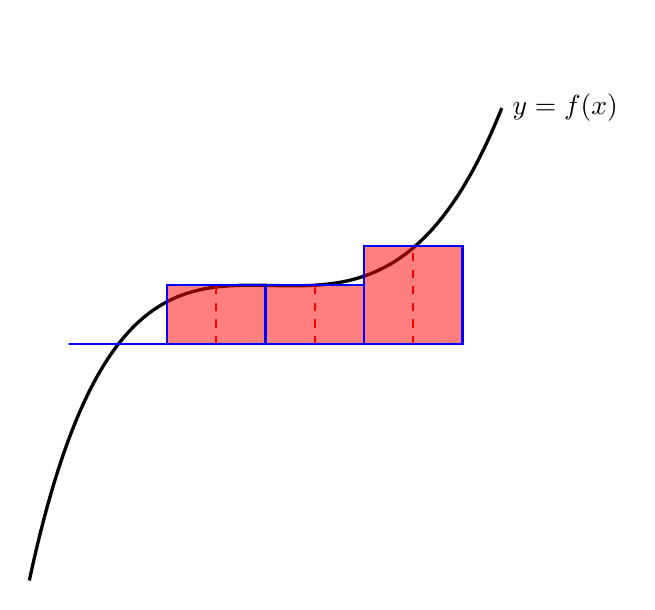
\begin{tikzpicture}
\YEaxis{4}{3};
\YExcoord{2.5}{b}
\YExcoord{-2.5}{a}
\draw[very thick] (-3,-3) .. controls (-1.5,4) and (1,-2) .. (3,3) node[right]{$y=f(x)$};
\draw[thick, red, dashed] (1.875,0)--(1.875,1.25);
\draw[thick, red, dashed] (-0.625,0)--(-0.625,0.75);
\draw[thick, red, dashed] (0.625,0)--(0.625,0.75);
\draw[thick, blue, fill =red, fill opacity=0.5] (-1.25,0) rectangle (0,.75);
\draw[thick, blue, fill =red, fill opacity=0.5] (0,0) rectangle (1.25,.75);
\draw[thick, blue, fill =red, fill opacity=0.5] (1.25,0) rectangle (2.5,1.25);
\draw[thick, blue, fill =red, fill opacity=0.5] (-2.5,0) rectangle (-1.25,0);
\end{tikzpicture}
\end{center}

\end{answer}
\begin{solution}
The index of the sum runs from 1 to 4: the first, second, third, and fourth rectangles. So, we have four rectangles in our Riemann sum. Let's start by drawing in the intervals along the $x$-axis taken up by these four rectangles. Note each has the same width: $\dfrac{b-a}{4}$.
\begin{center}
\begin{tikzpicture}
\YEaxis{4}{3};
\YExcoord{2.5}{b}
\YExcoord{-2.5}{a}
\draw[very thick] (-3,-3) .. controls (-1.5,4) and (1,-2) .. (3,3) node[right]{$y=f(x)$};
\draw[thick, blue] (-2.5,.2)--(-2.5,-.25);
\draw[thick, blue] (-1.25,.2)--(-1.25,-.25);
\draw[thick, blue] (0,.2)--(0,-.25);
\draw[thick, blue] (1.25,.2)--(1.25,-.25);
\draw[thick, blue] (2.5,.2)--(2.5,-.25);
\end{tikzpicture}
\end{center}

Since this is a midpoint Riemann sum, the height of each rectangle is given by the $y$-value of the function in the midpoint of the interval. So, now let's find the height of the function at the midpoints of each of the four intervals.

\begin{center}
\begin{tikzpicture}
\YEaxis{4}{3};
\YExcoord{2.5}{b}
\YExcoord{-2.5}{a}
\draw[very thick] (-3,-3) .. controls (-1.5,4) and (1,-2) .. (3,3) node[right]{$y=f(x)$};
\draw[thick, blue] (-2.5,.2)--(-2.5,-.25);
\draw[thick, blue] (-1.25,.2)--(-1.25,-.25);
\draw[thick, blue] (0,.2)--(0,-.25);
\draw[thick, blue] (1.25,.2)--(1.25,-.25);
\draw[thick, blue] (2.5,.2)--(2.5,-.25);
\draw[thick, red] (-1.875,-.2)--(-1.875,0);
\draw[thick, red] (1.875,-.2)--(1.875,1.25);
\draw[thick, red] (-0.625,-.2)--(-0.625,0.75);
\draw[thick, red] (0.625,-.2)--(0.625,0.75);
\end{tikzpicture}
\end{center}

The left-most interval has a height of about 0, so it gives a ``trivial" rectangle with no height and no area. The middle two intervals have rectangles of about the same height, and the right-most interval has the highest rectangle.

\begin{center}
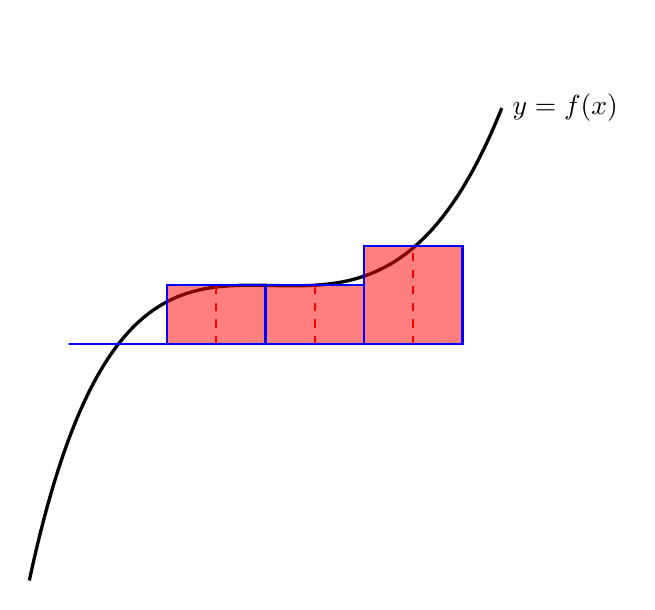
\begin{tikzpicture}
\YEaxis{4}{3};
\YExcoord{2.5}{b}
\YExcoord{-2.5}{a}
\draw[very thick] (-3,-3) .. controls (-1.5,4) and (1,-2) .. (3,3) node[right]{$y=f(x)$};
\draw[thick, red, dashed] (1.875,0)--(1.875,1.25);
\draw[thick, red, dashed] (-0.625,0)--(-0.625,0.75);
\draw[thick, red, dashed] (0.625,0)--(0.625,0.75);
\draw[thick, blue, fill =red, fill opacity=0.5] (-1.25,0) rectangle (0,.75);
\draw[thick, blue, fill =red, fill opacity=0.5] (0,0) rectangle (1.25,.75);
\draw[thick, blue, fill =red, fill opacity=0.5] (1.25,0) rectangle (2.5,1.25);
\draw[thick, blue, fill =red, fill opacity=0.5] (-2.5,0) rectangle (-1.25,0);
\end{tikzpicture}
\end{center}
\end{solution}



%%%%%%%%%%%%%%%%%%%

\begin{question}[M105 2015A]
$\displaystyle \sum_{k=1}^4 f(1+k)\cdot 1$ is a left Riemann sum for a function $f(x)$ on the interval $[a,b]$ with $n$ subintervals. Find the values of $a$, $b$ and $n$.
\end{question}

\begin{hint}
Write out the general formula for the left Riemann sum from Definition~\eref{CLP101}{def:INTthreeRiemannSums} in the CLP-2 text and
choose $a$, $b$ and $n$ to make it match the given sum.
\end{hint}

\begin{answer}
$n=4$, $a=2$, and $b=6$
\end{answer}

\begin{solution}
In general, the {left} Riemann sum for the integral $\int_a^b f(x)\,\,\dee{x}$
is of the form
\begin{align*}
\sum_{k=1}^n f\left(a+(k-1)\frac{b-a}{n}\right)\frac{b-a}{n}
\end{align*}

\begin{itemize}
\item
To get the limits of summation to match the given sum, we need $n=4$.
\item
Then to get the factor multiplying $f$ to match that in the given sum,
we need $\frac{b-a}{n}=1$, so $b-a=4$.
\item Finally, to get the argument of $f$ to match that in the given sum,
we need
\begin{align*}
a+(k-1)\frac{b-a}{n}=a-\frac{b-a}{n} +k\frac{b-a}{n}=1+k
\end{align*}
Subbing in $n=4$ and $b-a=4$ gives
$a-1 +k=1+k$, so $a=2$ and $b=6$.
\end{itemize}
\end{solution}

%%%%%%%%%%%%%%%%%%%%


\begin{question}\label{1.1RiemannInterp}
Draw a picture illustrating the area given by the following Riemann sum.
\[\sum_{i=1}^3 2\cdot\left(5+2i\right)^2 \]
\end{question}
\begin{hint}
Since the sum runs from 1 to 3, there are three intervals. Suppose $2 = \Delta x = \frac{b-a}{n}$. You may assume the sum given is a right Riemann sum (as opposed to left or midpoint).
\end{hint}
\begin{answer}
One answer is below, but other interpretations exist.


\begin{center}
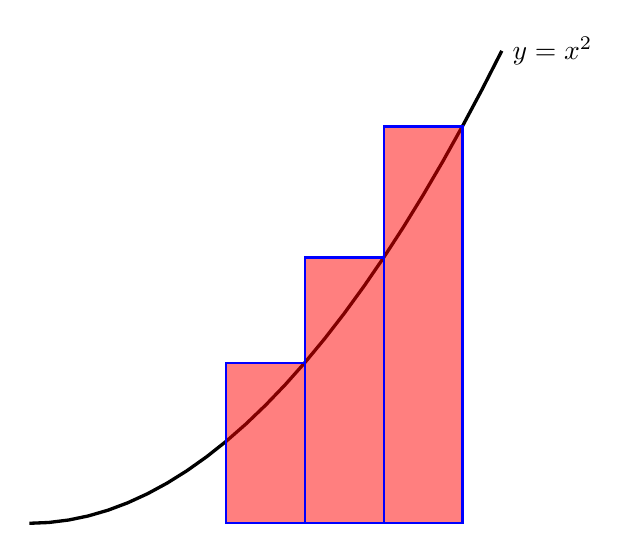
\begin{tikzpicture}
\YEaaxis{1}{7}{1}{7};
\foreach \x in {5,7,9,11}{
	\YExcoord{\x/2}{\x}}
\foreach \x in {7,9,11}{
	\MULTIPLY{\x}{\x}{\y}
	\YEycoord{\y/24}{\y}}
\draw[very thick] plot[domain=0:6] (\x,{\x*\x/6}) node[right]{$y=x^2$};
\draw[blue, thick, fill =red, fill opacity=0.5] (2.5,0) rectangle (3.5,2.04)
 (3.5,0) rectangle (4.5,3.375)
  (4.5,0) rectangle (5.5,5.04);
\end{tikzpicture}
\end{center}

\end{answer}
\begin{solution}
The general form of a Riemann sum is $\displaystyle\sum_{i=1}^n \Delta x \cdot f(x_i^*)$, where $\Delta x = \frac{b-a}{n}$ is the width of each rectangle, and $f(x_i^*)$ is the height.

There are different ways to interpret the given sum as a Riemann sum. The most obvious is given in Solution 1. You may notice that we make some convenient assumptions in this solution about values for $\Delta x$ and $a$, and we assume the sum is a right Riemann sum. Other visualizations of the sum arise from making more exotic choices. Some of these are explored in Solutions 2-4.

All cases have three rectangles, and the three rectangles will have the same areas: 98, 162, and 242 square units, respectively. This is because the terms of the given sum simplify to $98+162+242$.

\begin{description}
\item[Solution 1:]$ $
\begin{itemize}
\item Because the index runs from $1$ to $3$, there are three intervals: $n=3$.

\item Looking at our sum, it seems reasonable to interpret $\Delta x = 2$. Then, since $n=3$, we conclude $\frac{b-a}{3}=2$, hence $b-a=6$.

\item If $\Delta x = 2$, then $f(x_i^*)=\left(5+2i\right)^2$. Recall that $x_i^*$ is the $x$-coordinate we use to decide the height of the $i$th rectangle. In a right Riemann sum, $x_i^* = a+i\cdot\Delta x$. So, using $2=\Delta x$, we can let $f(x_i^*)=f(a+2i)=\left(5+2i\right)^2$. This fits with the function $f(x)=x^2$, and $a=5$.
\item Since $b-a=6$, and $a=5$, this tells us $b=11$
\end{itemize}

To sum up, we can interpret the Riemann sum as a right Riemann sum, with three intervals, of the function $f(x)=x^2$ from $x=5$ to $x=11$.


\begin{center}
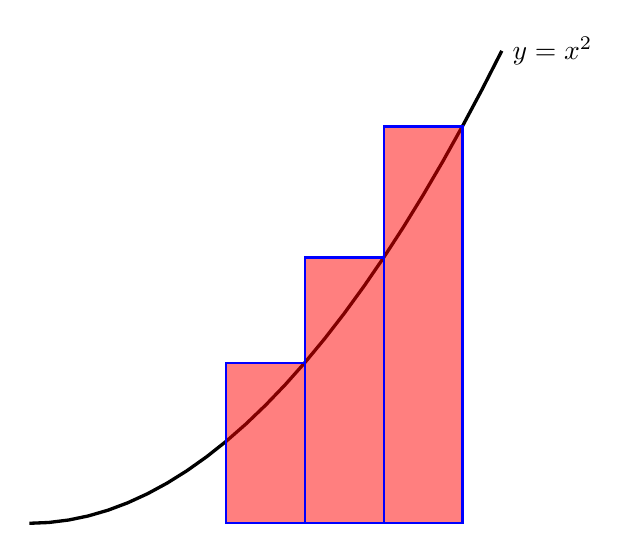
\begin{tikzpicture}
\YEaaxis{1}{7}{1}{7};
\foreach \x in {5,7,9,11}{
	\YExcoord{\x/2}{\x}}
\foreach \x in {7,9,11}{
	\MULTIPLY{\x}{\x}{\y}
	\YEycoord{\y/24}{\y}}
\draw[very thick] plot[domain=0:6] (\x,{\x*\x/6}) node[right]{$y=x^2$};
\draw[blue, thick, fill =red, fill opacity=0.5] (2.5,0) rectangle (3.5,2.04)
 (3.5,0) rectangle (4.5,3.375)
  (4.5,0) rectangle (5.5,5.04);
\end{tikzpicture}
\end{center}

\item[Solution 2: We could have chosen a different value for $\Delta x$.]
$ $
\begin{itemize}
\item The index of the sum runs from 1 to 3, so we have $n=3$.
\item We didn't have to interpret $\Delta x$ as 2--that was just the path of least resistance. We could have chosen it to be any other number--for the sake of argument, let's say $\Delta x=10$. (Positive numbers are easiest to interpret, but negatives are technically allowed as well.)

\item Then $10=\frac{b-a}{n}=\frac{b-a}{3}$, so $b-a=30$.
\item Let's use the paradigm of a right Riemann sum, and match up the terms of the sum given in the problem to the terms in the definition:
\begin{align*}
\Delta x \cdot f\left(a+i\cdot \Delta x\right)&= 2\cdot\left(5+2i\right)^2\\
10 \cdot f(a+10i)&= 2\cdot\left(5+2i\right)^2\\
f(a+10i)&=\frac{1}{5}\cdot\left(5+2i\right)^2\\
f(a+10i)&=\frac{1}{5}\cdot\left(5+\frac{1}{5}\cdot 10i\right)^2
\end{align*}
\item The easiest value of $a$ in this case is  $a=0$. Then $f(\textcolor{red}{10i}) = \frac{1}{5}\cdot\left(5+\frac{1}{5}\cdot \textcolor{red}{10i}\right)^2$, so $f(\textcolor{red}{x})= \frac{1}{5}\cdot\left(5+\frac{1}{5}\cdot \textcolor{red}{x}\right)^2$.
\item If $a=0$ and $b-a=30$, then $b=30$.
\item To sum up: $n=3$, $a=0$, $b=30$, $\Delta x = 10$, and $f(x)= \frac{1}{5}\cdot\left(5+\frac{x}{5} \right)^2$.

\begin{center}
\begin{tikzpicture}
\clip (-1.5,-1.5) rectangle (10,4);
\YEaaxis{1}{7}{1}{3};
\foreach \x in {10,20,30}{
	\YExcoord{\x/5}{\x}}
 \YEycoord{0.98}{\frac{49}{5}}
\YEycoord{1.62}{\frac{81}{5}}
\YEycoord{2.42}{\frac{121}{5}}
\draw[very thick] plot[domain=-2:35, xscale=.2, yscale=0.1] (\x,{.2*(5+\x/5)*(5+\x/5)}) ;
\draw (7,3)node[right]{$y=\frac{1}{5}\left(5+\frac{x}{5}\right)^2$};
\draw[blue, thick, fill =red, fill opacity=0.5] (0,0) rectangle (2,0.98)
 (2,0) rectangle (4,1.62)
  (4,0) rectangle (6,2.42);
\end{tikzpicture}
\end{center}
By changing $\Delta x$, we changed the \emph{widths} of the rectangles.
The rectangles in this picture are wider and shorter than the rectangles in Solution 1. Their \emph{areas} are the same: 98, 162, and 242.
\end{itemize}
\item[Solution 3: We could have chosen a different value of $a$.]
$ $
\begin{itemize}
\item Suppose $\Delta x = 2$,  and we interpret our sum as a right Riemann sum, but we didn't assume $a=5$. We could have chosen $a$ to be any number--say, $a=1$.

\item   Let's match up what we're given in the problem to what we're given as a definition:
\begin{align*}
\Delta x \cdot f\left(a+i\cdot\Delta x\right)&=2\cdot\left(5+2i\right)^2\\
2 \cdot f\left(1+2i\right)&=2\cdot\left(5+2i\right)^2\\
f\left(1+2i\right)&=\left(5+2i\right)^2\\
f\left(1+2i\right)&=\left(4+1+2i\right)^2
\end{align*}
\item Since $f(\textcolor{red}{1+2i})=\left(4+\textcolor{red}{1+2i}\right)^2$, we have $f(\textcolor{red}{x})=\left(4+\textcolor{red}{x}\right)^2$
\item Since $a=1$ and $\frac{b-a}{3}=2$, in this case $b=7$.
\item To sum up: $n=3$, $a=1$, $b=7$, $\Delta x=2$, and $f(x)=(4+x)^2$.
\begin{center}
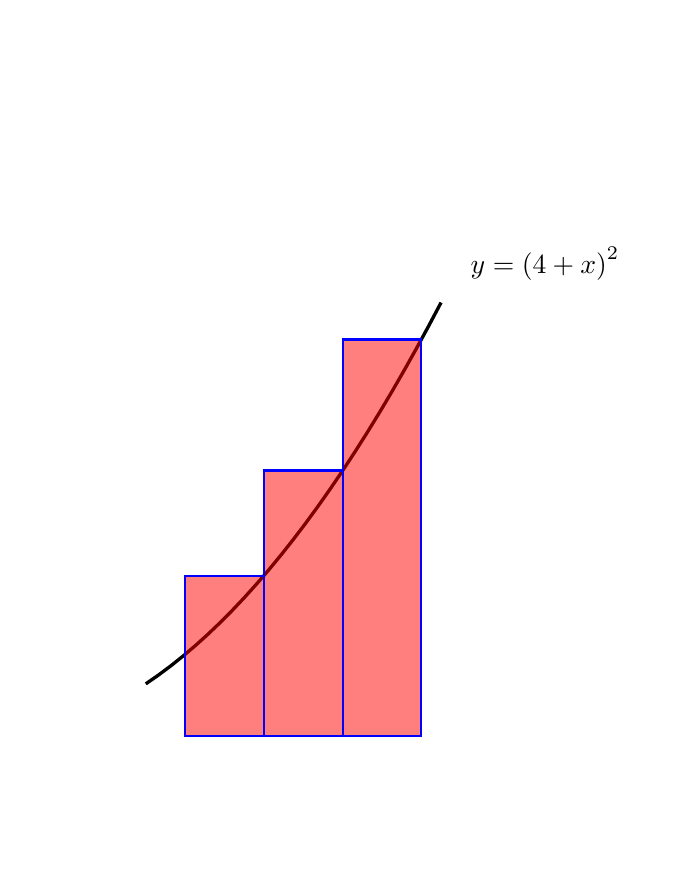
\begin{tikzpicture}
\clip (-1.5,-1.5) rectangle (6.5,9);
\YEaaxis{1}{4}{1}{6.5};
\foreach \x in {1,3,5,7}{
	\YExcoord{\x/2}{\x}}
\foreach \x in {7,9,11}{
	\MULTIPLY{\x}{\x}{\y}
	\YEycoord{\y/24}{\y}}
\draw[very thick] plot[domain=0:7.5, xscale=0.5, yscale=1/24] (\x,{(4+\x)*(4+\x)}) ;
\draw (4,6) node[right]{$y=\left(4+x\right)^2$};
\draw[blue, thick, fill =red, fill opacity=0.5] (.5,0) rectangle (1.5,2.04)
 (1.5,0) rectangle (2.5,3.375)
  (2.5,0) rectangle (3.5,5.04);
\end{tikzpicture}
\end{center}
This picture is a lot like the picture in Solution 1, but shifted to the left.
By changing $a$, we changed the \emph{left endpoint} of our region.
\end{itemize}

\item[Solution 4: We could have chosen a different kind of Riemann sum.]
$ $
\begin{itemize}
\item We didn't have to assume that we were dealing with a \emph{right} Riemann sum. Suppose $\Delta x =2$, and we have a \emph{midpoint} Riemann sum.

\item Let's match up what we're given in the problem with what we're given in the definition:
\begin{align*}
\Delta x \cdot f\left(a+\left(i-\tfrac{1}{2}\right)\Delta x\right)&=2\cdot\left(5+2i\right)^2\\
2 \cdot f\left(a+\left(i-\tfrac{1}{2}\right)2\right)&=2\cdot\left(5+2i\right)^2\\
f\left(a+\left(i-\tfrac{1}{2}\right)2\right)&=\left(5+2i\right)^2\\
f\left(a+2i-1\right)&=\left(5+2i\right)^2\\
f\left((a-1)+2i\right)&=\left(5+2i\right)^2
\end{align*}
\item It is now convenient to set $a-1=5$, hence $a=6$.
\item Then $f(\textcolor{red}{5+2i})=(\textcolor{red}{5+2i})^2$, so $f(\textcolor{red}{x})=\textcolor{red}{x}^2$
\item Since $2=\frac{b-a}{3}$ and $a=6$, we see $b=12$.
\item To sum up: $n=3$, $a=6$, $b=12$, $\Delta x = 2$, and $f(x)=x^2$.
\begin{center}
\begin{tikzpicture}
\clip (-1.5,-1.5) rectangle (9,7);
\YEaaxis{1}{7}{1}{6.5};
\foreach \x in {6,8,10,12}{
	\YExcoord{\x/2}{\x}}
\foreach \x in {7,9,11}{
	\MULTIPLY{\x}{\x}{\y}
	\YEycoord{\y/24}{\y}
	\draw[red, dashed, very thick] (\x/2,0)--(\x/2,\y/24);}
\draw[very thick] plot[domain=0:12, xscale=0.5, yscale=1/24] (\x,{\x*\x}) ;
\draw (6.5,5.5) node[right]{$y=x^2$};
\draw[blue, thick, fill =red, fill opacity=0.5] (3,0) rectangle (4,2.04)
 (4,0) rectangle (5,3.375)
  (5,0) rectangle (6,5.04);
\end{tikzpicture}
\end{center}
By choosing to interpret our sum as a midpoint Riemann sum instead of a right Riemann sum, we changed where our rectangles intersect the graph $y=f(x)$:  instead of the graph hitting the right corner of the rectangle, it hits in the middle.
\end{itemize}
\end{description}
\end{solution}


\begin{question}
Draw a picture illustrating the area given by the following Riemann sum.
\[\sum_{i=1}^5 \frac{\pi}{20}\cdot \tan\left(\frac{\pi (i-1)}{20}\right)\]
\end{question}
\begin{hint}
Let $\Delta x = \dfrac{\pi}{20}$. Then what is $b-a$?
\end{hint}
\begin{answer}
Many interpretations are possible--see the solution to Question~\ref{1.1RiemannInterp} for a more thorough discussion--but the most obvious is given below.

\begin{center}
\begin{tikzpicture}
\YEaaxis{1}{5.5}{1}{6};
\foreach \x in {2,...,5}{
	\YExcoord{\x}{\frac{\x \pi}{20}}}
	\YExcoord{1}{\frac{ \pi}{20}}
\draw[very thick] plot[domain=0:0.78, xscale=6.25, yscale=6.25] (\x,{tan(\x r)}) ;
\draw (5.25,6.225) node[right]{$y=\tan x$};
\draw[blue, thick, fill =red, fill opacity=0.5] (0,0) rectangle (1,0)
(1,0) rectangle (2,0.99)
 (2,0) rectangle (3,2.03)
  (3,0) rectangle (4,3.18)
  (4,0) rectangle (5,4.54);
\end{tikzpicture}
\end{center}

\end{answer}
\begin{solution}
Many interpretations are possible--see the solution to Question~\ref{1.1RiemannInterp} for a more thorough discussion--but the most obvious is given below. Recall the definition of a left Riemann sum:
\[\sum_{i=1}^n \Delta x \cdot f\left(a+(i-1)\Delta x\right)\]
We chose a left Riemann sum instead of right or midpoint because our given sum has $(i-1)$ in it, rather than $(i-\frac{1}{2})$ or simply $i$.
\begin{itemize}
\item Since the sum has five terms ($i$ runs from 1 to 5), there are 5 rectangles. That is, $n=5$.
\item In the definition of the Riemann sum, note that the term $\Delta x$ appears twice: once multiplied by the entire term, and once multiplied by $i-1$. So, a convenient choice for $\Delta x$ is $\frac{\pi}{20}$, because this is the constant that is both multiplied at the start of the term, and multiplied by $i-1$.
\item Since $\dfrac{\pi}{20}=\Delta x = \dfrac{b-a}{n} = \dfrac{b-a}{5}$, we see $b-a=\dfrac{5\pi}{20}=\dfrac{\pi}{4}$.
\item We match the terms in the definition with the terms in the problem:
\begin{align*}
f(a+(i-1)\Delta x) & = \tan\left(\frac{\pi (i-1)}{20}\right)\\
f\left(a+(i-1)\frac{\pi}{20}\right) & = \tan\left((i-1)\frac{\pi }{20}\right)
\end{align*}
So, we choose $a=0$ and $f(x) = \tan x$.
\item Since $a=0$ and $b-a=\frac{\pi}{4}$, we see $b=\frac{\pi}{4}$.
\end{itemize}


\begin{center}
\begin{tikzpicture}
\YEaaxis{1}{5.5}{1}{6};
\foreach \x in {2,...,5}{
	\YExcoord{\x}{\frac{\x \pi}{20}}}
	\YExcoord{1}{\frac{ \pi}{20}}
\draw[very thick] plot[domain=0:0.78, xscale=6.25, yscale=6.25] (\x,{tan(\x r)}) ;
\draw (5.25,6.225) node[right]{$y=\tan x$};
\draw[blue, thick, fill =red, fill opacity=0.5] (0,0) rectangle (1,0)
(1,0) rectangle (2,0.99)
 (2,0) rectangle (3,2.03)
  (3,0) rectangle (4,3.18)
  (4,0) rectangle (5,4.54);
\end{tikzpicture}
\end{center}
We note that the first rectangle of the five is a ``trivial" rectangle, with height (and area) 0.
\end{solution}



%%%%%%%%%%%%%%%%%%%



\begin{Mquestion}[M105 2013A]\label{1.1Riemannb}
Fill in the blanks with right, left, or midpoint;
an interval; and a value of n.

\begin{enumerate}[(a)]
\item[]
$\sum\limits_{k=0}^3 f (1.5 + k) \cdot 1$ is a
$\underline{\ \ \ \ \ \ \ \ \ \ \ \ }$
Riemann sum for $f$ on the interval
$[\,\underline{\ \ \ \ \ \ }\ ,\ \underline{\ \ \ \ \ \ }\,]$ with
$n =\underline{\ \ \ \ \ }$.
\end{enumerate}
\end{Mquestion}

\begin{hint}
Notice that the index starts at $k=0$, instead of $k=1$.
Write out the given sum explicitly without using summation notation, and sketch where the rectangles would fall on a graph of $y=f(x)$.
%Also write out the first few terms in the sums in the three bullets of
%Definition \eref{CLP101}{def:INTthreeRiemannSums} in the
%\href{http://www.math.ubc.ca/%7Efeldman/m101/clp/clp_notes_101.pdf}{CLP-II text}.
%CLP-2 text.
Then try to identify $b-a$, and $n$,
followed by ``right'', ``left'', or ``midpoint'', and finally $a$.
\end{hint}

\begin{answer}
Three answers are possible.
It is a
midpoint Riemann sum for $f$ on the interval $[1,5]$ with $n =4$.
It is also a left Riemann sum for $f$ on the interval $[1.5,5.5]$ with $n =4$.
It is also a right Riemann sum for $f$ on the interval $[0.5,4.5]$ with $n =4$.
\end{answer}

\begin{solution}
Since there are four terms in the sum, $n=4$. (Note the sum starts at $k=0$, instead of $k=1$.) Since the function is multiplied by 1, $1=\Delta x=\dfrac{b-a}{n}=\dfrac{b-a}{4}$, hence $b-a=4$.

We can choose to view the given sum as a left, right, or midpoint Riemann sum. The choice we make determines the interval. Note that the heights of the rectangles are determined when $x = 1.5,\, 2.5,\, 3.5,$ and $4.5$.
\begin{center}
\begin{tikzpicture}
\YEaaxis{.5}{5.5}{.5}{5}
\foreach \k in {1,...,4}{
	\YEycoord{\k}{f(\k.5)}
	\ADD{\k}{1}{\l}
	\draw[thick, fill=blue, fill opacity=0.5] (\k,0) rectangle (\l,\k);}
\end{tikzpicture}
\end{center}
\begin{description}
\item[Option 1: right Riemann sum]
If our sum is a right Riemann sum, then we take the heights of the rectangles from the right endpoint of each interval.
\begin{center}
\begin{tikzpicture}
\YEaaxis{.5}{5.5}{.5}{5}
\foreach \k in {1,...,4}{
	\YEycoord{\k}{f(\k.5)}
	\ADD{\k}{1}{\l}
	\draw[thick, fill=blue, fill opacity=0.5] (\k,0) rectangle (\l,\k);
	\draw(\l,\k)node[vertex]{};
	\YExcoord{\l}{\k.5}}
\draw[thick] (2,1)--(5,4);
\end{tikzpicture}
\end{center}

Then $a=0.5$ and $b=4.5$. Therefore: $\sum\limits_{k=0}^3 f (1.5 + k) \cdot 1$ is a right Riemann sum on the interval $[0.5,4.5]$ with $n=4$.
\item[Option 2: left Riemann sum]
If our sum is a left Riemann sum, then we take the heights of the rectangles from the left endpoint of each interval.

\begin{center}
\begin{tikzpicture}
\YEaaxis{.5}{5.5}{.5}{5}
\foreach \k in {1,...,4}{
	\YEycoord{\k}{f(\k.5)}
	\ADD{\k}{1}{\l}
	\draw[thick, fill=blue, fill opacity=0.5] (\k,0) rectangle (\l,\k);
	\draw(\k,\k)node[vertex]{};
	\YExcoord{\k}{\k.5}}
	\draw[thick] (1,1)--(4,4);
\end{tikzpicture}
\end{center}

Then $a=1.5$ and $b=5.5$. Therefore: $\sum\limits_{k=0}^3 f (1.5 + k) \cdot 1$ is a left Riemann sum on the interval $[1.5,5.5]$ with $n=4$.
\item[Option 3: midpoint Riemann sum]
If our sum is a midpoint Riemann sum, then we take the heights of the rectangles from the midpoint of each interval.

\begin{center}
\begin{tikzpicture}
\YEaaxis{.5}{5.5}{.5}{5}
\foreach \k in {1,...,4}{
	\YEycoord{\k}{f(\k.5)}
	\ADD{\k}{1}{\l}
	\ADD{\k}{.5}{\m}
	\draw[thick, fill=blue, fill opacity=0.5] (\k,0) rectangle (\l,\k);
	\draw(\m,\k)node[vertex]{};
	\YExcoord{\m}{\k.5}}
\draw[thick] (1.5,1)--(4.5,4);
\end{tikzpicture}
\end{center}

Then $a=1$ and $b=5$. Therefore: $\sum\limits_{k=0}^3 f (1.5 + k) \cdot 1$ is a midpoint Riemann sum on the interval $[1,5]$ with $n=4$.

\end{description}
\end{solution}
%%%%%%%%%%%%%%%%%%%

\begin{question}
Evaluate the following integral by interpreting it as a signed area, and using geometry:
\[\int_0^5 x \,\dee{x}\]
\end{question}
\begin{hint}
The area is a triangle.
\end{hint}
\begin{answer}
$\dfrac{25}{2}$
\end{answer}
\begin{solution}
The area in question is a triangle with base 5 and height 5, so its area is $\dfrac{25}{2}$.
\begin{center}
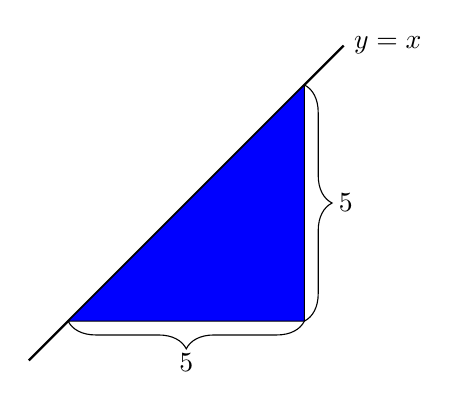
\begin{tikzpicture}
\YEaaxis{1}{4}{1}{4}
\draw[thick] (-.5,-.5)--(3.5,3.5) node[right]{$y=x$};
\draw[fill=blue] (0,0)--(3,3)--(3,0)--cycle;
\YEycoord{3}{5}
\draw[decorate, decoration={brace, amplitude=10pt}] (3,0)--(0,0) node[midway, yshift=-15pt]{$5$};
\draw[decorate, decoration={brace, amplitude=10pt}] (3,3)--(3,0) node[midway, xshift=15pt]{$5$};
\end{tikzpicture}
\end{center}
\end{solution}



\begin{Mquestion}
Evaluate the following integral by interpreting it as a signed area, and using geometry:
\[\int_{-2}^5 x \,\dee{x}\]
\end{Mquestion}
\begin{hint} There is one triangle of positive area, and one of negative area.
\end{hint}
\begin{answer}
$\dfrac{21}{2}$
\end{answer}
\begin{solution}

There is a positive and a negative portion of this area. The positive area is a triangle with base 5 and height 5, so area $\dfrac{25}{2}$ square units. The negative area is a triangle with base $2$ and height $2$, so negative area $\dfrac{4}{2}=2$ square units. So, the net area is $\dfrac{25}{2}-\dfrac{4}{2}=\dfrac{21}{2}$ square units.
\begin{center}
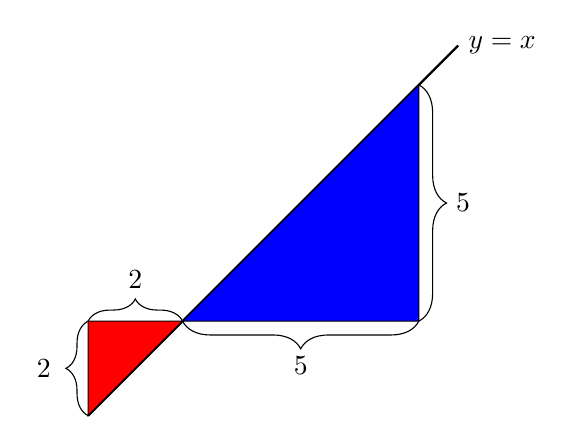
\begin{tikzpicture}
\YEaaxis{2}{4}{2}{4}
\draw[thick] (-1.2,-1.2)--(3.5,3.5) node[right]{$y=x$};
\draw[fill=blue] (0,0)--(3,3)--(3,0)--cycle;
\draw[fill=red] (0,0)--(-1.2,-1.2)--(-1.2,0)--cycle;
\YEycoord{3}{5}
\draw[decorate, decoration={brace, amplitude=10pt}] (3,0)--(0,0) node[midway, yshift=-16pt]{$5$};
\draw[decorate, decoration={brace, amplitude=10pt}] (3,3)--(3,0) node[midway, xshift=16pt]{$5$};
\draw[decorate, decoration={brace, amplitude=8pt}] (-1.2,0)--(0,0) node[midway, yshift=15pt]{$2$};
\draw[decorate, decoration={brace, amplitude=8pt}] (-1.2,-1.2)--(-1.2,0) node[midway, xshift=-16pt]{$2$};
\end{tikzpicture}
\end{center}
\end{solution}




%%%%%%%%%%%%%%%%%%
\subsection*{\Procedural}
%%%%%%%%%%%%%%%%%%

\begin{question}[M105 2014A]
Use sigma notation to write the midpoint Riemann sum for $f(x)=x^8$ on $[5,15]$
with $n=50$. Do not evaluate the Riemann sum.
\end{question}

\begin{hint}
Review Definition  \eref{CLP101}{def:INTthreeRiemannSums} in the
%\href{http://www.math.ubc.ca/%7Efeldman/m101/clp/clp_notes_101.pdf}{CLP 101 notes}
CLP-2 text.
\end{hint}

\begin{answer}
$\sum\limits_{i=1}^{50} \Big(5+\big(i-\nicefrac{1}{2}\big)\frac{1}{5}\Big)^8
\ \frac{1}{5}$
\end{answer}

\begin{solution}
In general, the midpoint Riemann sum is given by
\begin{align*}
\sum_{i=1}^n f\Big(a+\big(i-\nicefrac{1}{2}\big)\De x\Big)\ \De x \, ,
\qquad \mbox{where } \De x = \frac{b-a}{n}.
\end{align*}
In this problem we are told that $f(x)=x^8$, $a=5$, $b=15$ and $n=50$,
so that $\De x = \frac{b-a}{n} = \frac{1}{5}$ and the desired Riemann sum is:
\begin{align*}
\sum_{i=1}^{50} \Big(5+\big(i-\nicefrac{1}{2}\big)\frac{1}{5}\Big)^8
\ \frac{1}{5}
\end{align*}
\end{solution}
%%%%%%%%%%%%%%%%%%%




\begin{question}[2016Q1]
Estimate $\displaystyle\int_{-1}^5 x^3\,\,\dee{x}$ using three approximating rectangles
and left hand end points.
\end{question}

%\begin{hint}
%\end{hint}

\begin{answer}
$54$
\end{answer}

\begin{solution}
The given integral has interval of integration going from $a=-1$ to $b=5$.
So when we use three approximating rectangles, all of the same width, the common width
is $\Delta x=\frac{b-a}{n} = 2$. The first rectangle has left  endpoint $x_0=a=-1$,
the second has left hand endpoint $x_1=a+\Delta x=1$, and the third has left hand end point
$x_2=a+2\Delta x=3$. So
\begin{align*}
\int_{-1}^5 x^3\,\,\dee{x}
\approx \big[f(x_0)+f(x_1)+f(x_2)\big]\Delta x
=\big[(-1)^3+1^3+3^3\big]\times2
=54
\end{align*}
\end{solution}

%%%%%%%%%%%%%%%%%



\begin{Mquestion}[2016Q1]
Let $f$ be a function on the whole real line.  Express
$\displaystyle\int_{-1}^{7}f(x)\,\,\dee{x}$ as a limit of Riemann sums, using the
right endpoints.
\end{Mquestion}

\begin{hint}
You'll want the limit as $n$ goes to infinity of a sum with $n$ terms. If you're having a hard time coming up with the sum in terms of $n$, try writing a sum with a finite number of terms of your choosing. Then, think about how that sum would change if it had $n$ terms.
\end{hint}

\begin{answer}
$\displaystyle\int_{-1}^{7}f(x)\,\,\dee{x}=\displaystyle\lim_{n\to\infty}\displaystyle\sum_{i=1}^{n} f\left(-1+\frac{8i}{n}\right)\frac{8}{n}$
\end{answer}

\begin{solution}
In the given integral, the domain of integration runs from $a=-1$ to $b=7$.
So, we have $\Delta x = \frac{(b-a)}{n}= \frac{(7-(-1))}{n} = \frac{8}{n}$. The left-hand end of the first
subinterval is at $x_0=a=-1$. So, the right-hand end of the $i^{\rm th}$ interval
is at $x_i^* = -1+\frac{8i}{n}$. So:
\begin{align*}
\int_{-1}^{7}f(x)\,\,\dee{x}
=\lim_{n\to\infty}\sum_{i=1}^{n} f\left(-1+\frac{8i}{n}\right)\frac{8}{n}
\end{align*}

\end{solution}

%%%%%%%%%%%%%%%
\begin{question}[2016Q1]
The value of the following limit is equal to the area below a graph of $y=f(x)$, integrated over the interval $[0,b]$:
\begin{align*}
   \lim_{n \to \infty} \sum_{i=1}^{n} \frac{4}{n}
          \left[ \sin \left( 2 + \frac{4i}{n}\right)\right]^2
\end{align*}
Find $f(x)$ and $b$.
\end{question}

\begin{hint}
The main step is to express the given sum as the right Riemann sum,
\[\sum_{i=1}^{n} f(a+i\De x)\Delta  x.\]
Don't be afraid to guess $\De x$ and $f(x$)
(review Definition  \eref{CLP101}{def:INTthreeRiemannSums} in the
%\href{http://www.math.ubc.ca/%7Efeldman/m101/clp/clp_notes_101.pdf}{CLP 101 notes}
CLP-2 text).
Then write out explicitly $ \sum\limits_{i=1}^{n} f(a+i\De x)\Delta  x$
with your guess substituted in, and compare the result with the given sum.  Adjust your guess if they don't match.
\end{hint}

\begin{answer}
$f(x) = \sin^2 (2 + x)$ and $b=4$
\end{answer}

\begin{solution}
We identify the given sum as the right Riemann sum
$\sum\limits_{i=1}^{n} f(a+i\De x)\Delta  x$,
with $a=0$ (that's specified in the statement of the question). Since $\frac{4}{n}$ is multiplied in every term, and is also multiplied by $i$, we let
 $\Delta x = \frac{4}{n}$. Then $x_i^* = a+i\De x=\frac{4i}{n}$
and $f(x) = \sin^2 (2 + x)$. So, $b=a+n\De x=0+n\cdot\frac{4}{n}=4$.
\end{solution}
%%%%%%%%%%%%%%%%%%%

\begin{Mquestion}[M105 2102A]
For a certain function $f(x)$, the following equation holds:
\begin{equation*}
\lim_{n\rightarrow\infty}\sum\limits_{k=1}^n
\frac{k}{n^2}\sqrt{1-\frac{k^2}{n^2}}
=\int_0^1 f(x)\ \,\dee{x}
\end{equation*}
Find $f(x)$.
\end{Mquestion}

\begin{hint}
The main step is to express the given sum as the right Riemann sum
$\sum\limits_{k=1}^{n} f(a+k\De x)\Delta  x$.
Don't be afraid to guess $\De x$ and $f(x$)
(review Definition  \eref{CLP101}{def:INTthreeRiemannSums} in the
%\href{http://www.math.ubc.ca/%7Efeldman/m101/clp/clp_notes_101.pdf}{CLP 101 notes}
CLP-2 text).
Then write out explicitly $ \sum\limits_{k=1}^{n} f(a+k\De x)\Delta  x$
with your guess substituted in, and compare the result with the given sum.  Adjust your guess if they don't match.
\end{hint}

\begin{answer}
$f(x)=x\sqrt{1-x^2}$
\end{answer}

\begin{solution}
The given sum is of the form
\begin{align*}
\lim_{n\rightarrow\infty}\sum_{k=1}^n
             \frac{k}{n^2}\sqrt{1-\frac{k^2}{n^2}}
=\lim_{n\rightarrow\infty}\sum_{k=1}^n
            \left(\frac{1}{n}\right) \frac{k}{n}\sqrt{1-\left(\frac{k}{n}\right)^2}
=\lim_{n\rightarrow\infty}\sum_{k=1}^n \De x f(x_k^*)
\end{align*}
with $\De x=\frac{1}{n}$, $a=0$, $x_k^*=\frac{k}{n}=a+k\De x$
and $f(x)=x\sqrt{1-x^2}$.
Since $x_0^*=0$ and $x_n^*=1$, the right hand side is the definition
(using the right Riemann sum) of
$
\int_0^1 f(x)\,\,\dee{x}
$.

\end{solution}
%%%%%%%%%%%%%%%%%%%


\begin{question}[2016Q1]
Express $\displaystyle\lim_{n\to\infty}\displaystyle\sum_{i=1}^{n}
                       \frac{3}{n} e^{-i/n} \cos\left(\frac{3i}{n}\right)$
as a definite integral.
\end{question}

\begin{hint}
The main step is to express the given sum in the form $ \sum_{i=1}^{n} f(x_i^*)\Delta  x$.
Don't be afraid to guess $\De x$, $x_i^*$ (for either a left or a right or a  midpoint sum ---
review Definition  \eref{CLP101}{def:INTthreeRiemannSums} in the
%\href{http://www.math.ubc.ca/%7Efeldman/m101/clp/clp_notes_101.pdf}{CLP 101 notes}
CLP-2 text)
and $f(x$). Then write out explicitly $ \sum_{i=1}^{n} f(x_i^*)\Delta  x$ with your guess
substituted in, and compare the result with the given sum.  Adjust your guess if they don't match.
\end{hint}

\begin{answer}
$\int_0^3 e^{-x/3}\cos(x)\,\,\dee{x}$
\end{answer}

\begin{solution}
As $i$ ranges from $1$ to $n$, $3i/n$ range from $3/n$ to $3$ with jumps of
$\De x=3/n$, so this is
\begin{align*}
\lim_{n\to\infty}\displaystyle\sum_{i=1}^{n}
                       \frac{3}{n} e^{-i/n} \cos(3i/n)
=\lim_{n\to\infty} \sum_{i=1}^{n} f(x_i^*)\Delta  x
=\int_a^b f(x)\,\,\dee{x}
\end{align*}
where $x_i^* = 3i/n$, $f(x) = e^{-x/3}\cos(x)$, $a=x_0=0$ and $b=x_n=3$. Thus
\begin{align*}
\lim_{n\to\infty}\displaystyle\sum_{i=1}^{n}
                       \frac{3}{n} e^{-i/n} \cos(3i/n)
=\int_0^3 e^{-x/3}\cos(x)\,\,\dee{x}
\end{align*}

\end{solution}
%%%%%%%%%%%%%%%%%%%

\begin{question}[2012A, 2014D]
Let $\displaystyle R_n= \sum_{i=1}^{n}
                       \frac{i e^{i/n}}{n^2}$.
Express $\displaystyle\lim_{n\to\infty}R_n$
as a definite integral. \emph{Do not evaluate this integral.}
\end{question}

\begin{hint}
The main step is to express the given sum in the form
$\sum\limits_{i=1}^{n} f(x_i^*)\Delta  x$.
Don't be afraid to guess $\De x$, $x_i^*$ (probably, based on the symbol $R_n$,
assuming we have a right Riemann sum ---
review Definition  \eref{CLP101}{def:INTthreeRiemannSums} in the CLP-2 text)
and $f(x$). Then write out explicitly $ \sum\limits_{i=1}^{n} f(x_i^*)\Delta  x$ with
your guess substituted in, and compare the result with the given sum.
Adjust your guess if they don't match.
\end{hint}

\begin{answer}
$\displaystyle\int_0^1 x e^{x}\,\,\dee{x}$
\end{answer}

\begin{solution}
As $i$ ranges from $1$ to $n$, the exponent $\frac{i}{n}$ ranges from $\frac{1}{n}$ to $1$ with
jumps of $\De x=\frac{1}{n}$. So let's try $x_i^* =\frac{ i}{n}$, $\Delta x=\frac{1}{n}$. Then:
\begin{align*}
R_n= \sum_{i=1}^{n} \frac{i e^{i/n}}{n^2}
= \sum_{i=1}^{n} \frac{i}{n} e^{i/n} \frac{1}{n}
= \sum_{i=1}^{n} x_i^* e^{x_i^*} \Delta x
= \sum_{i=1}^{n} f(x_i^*) \Delta x
\end{align*}
with $f(x)= x e^x$, and the limit
\begin{align*}
\lim_{n\to\infty} R_n
=\lim_{n\to\infty} \sum_{i=1}^{n} f(x_i^*)\Delta  x
=\int_a^b f(x)\,\,\dee{x}
\end{align*}
Since we chose $x_i^* = \frac{i}{n} = 0+i\De x$, we let $a=0$. Then $\frac{1}{n}=\De x = \frac{b-a}{n}=\frac{b}{n}$ tells us $b=1$. Thus,
\begin{align*}
\lim_{n\to\infty}R_n
=\int_0^1 xe^{x}\,\,\dee{x}\,.
\end{align*}

\end{solution}
%%%%%%%%%%%%%%%%%%%


\begin{Mquestion}[2016A]
Express
$\displaystyle\lim_{n\rightarrow\infty} \bigg( \sum_{i=1}^n e^{-1-2i/n}\cdot \frac{2}{n} \bigg)$
as an integral in three different ways.
\end{Mquestion}

\begin{hint}
Try several different choices of $\De x$ and $x_i^*$.
\end{hint}

\begin{answer}
Possible answers include:\\[5pt] $\displaystyle\int\limits_0^2 e^{-1-x}\ \,\dee{x}$,\quad
                                $\displaystyle\int\limits_1^3 e^{-x}\ \,\dee{x}$, \quad
                                $2\displaystyle\int_{1/2}^{3/2} e^{-2x}\ \,\dee{x}$, \quad
and \quad
                                $2\displaystyle\int\limits_0^1 e^{-1-2x}\ \,\dee{x}$.
\end{answer}

\begin{solution}
\begin{description}
\item[Choice \#1:]
If we set $\De x = \frac{2}{n}$ and $x_i^*= \frac{2i}{n}$, i.e. $x_i^* = a + i\De x$ with $a=0$,
then
\begin{align*}
\lim_{n\rightarrow\infty} \bigg( \sum_{i=1}^n e^{-1-2i/n}\cdot \frac{2}{n} \bigg)
&=\lim_{n\rightarrow\infty} \bigg( \sum_{i=1}^n e^{-1-x_i^*}\De x \bigg) \hidewidth \\
&=\lim_{n\rightarrow\infty} \bigg( \sum_{i=1}^n f(x_i^*)\De x \bigg) &&\text{with $f(x) = e^{-1-x}$} \\
&=\int_a^b f(x)\,\,\dee{x}&&\text{with $a=x_0=0$ and $b=x_n=2$} \\
&=\int_0^2 e^{-1-x}\ \,\dee{x}
\end{align*}


\item[Choice \#2:]
If we set $\De x = \frac{2}{n}$ and $x_i^*= 1+\frac{2i}{n}$, i.e. $x_i^* = a + i\De x$
with $a=1$,
then
\begin{align*}
\lim_{n\rightarrow\infty} \bigg( \sum_{i=1}^n e^{-1-2i/n}\cdot \frac{2}{n} \bigg)
&=\lim_{n\rightarrow\infty} \bigg( \sum_{i=1}^n e^{-x_i^*}\De x \bigg) \hidewidth \\
&=\lim_{n\rightarrow\infty} \bigg( \sum_{i=1}^n f(x_i^*)\De x \bigg) &&\text{with $f(x) = e^{-x}$} \\
&=\int_a^b f(x)\,\,\dee{x}&&\text{with $a=x_0=1$ and $b=x_n=3$} \\
&=\int_1^3 e^{-x}\ \,\dee{x}
\end{align*}

\item[Choice \#3:]
If we set $\De x = \frac{1}{n}$ and $x_i^*= \frac{i}{n}$, i.e. $x_i^* = a + i\De x$ with $a=0$,
then
\begin{align*}
\lim_{n\rightarrow\infty} \bigg( \sum_{i=1}^n e^{-1-2i/n}\cdot \frac{2}{n} \bigg)
&=\lim_{n\rightarrow\infty} \bigg( \sum_{i=1}^n e^{-1-2x_i^*}\ 2\De x \bigg) \hidewidth \\
&=\lim_{n\rightarrow\infty} \bigg( \sum_{i=1}^n f(x_i^*)\De x \bigg)
                       &&\text{with $f(x) = 2e^{-1-2x}$} \\
&=\int_a^b f(x)\,\,\dee{x}&&\text{with $a=x_0=0$ and $b=x_n=1$} \\
&=2\int_0^1 e^{-1-2x}\ \,\dee{x}
\end{align*}

\item[Choice \#4:]
If we set $\De x = \frac{1}{n}$ and $x_i^*= \frac{1}{2}+\frac{i}{n}$, i.e. $x_i = a + i\De x$
with $a=\frac{1}{2}$,
then
\begin{align*}
\lim_{n\rightarrow\infty} \bigg( \sum_{i=1}^n e^{-1-2i/n}\cdot \frac{2}{n} \bigg)
&=\lim_{n\rightarrow\infty} \bigg( \sum_{i=1}^n e^{-2x_i}\ 2\De x \bigg) \hidewidth \\
&=\lim_{n\rightarrow\infty} \bigg( \sum_{i=1}^n f(x_i^*)\De x \bigg)
                       &&\text{with $f(x) = 2e^{-2x}$} \\
&=\int_a^b f(x)\,\,\dee{x}&&\text{with $a=x_0=\frac{1}{2}$ and $b=x_n=\frac{3}{2}$} \\
&=2\int_{1/2}^{3/2} e^{-2x}\ \,\dee{x}
\end{align*}

\end{description}

\end{solution}
%%%%%%%%%%%%%%%%%%%


\Instructions{Questions~\ref{1.1geoma} and \ref{1.1geomb} use the formula for a geometric sum, Equation~\eref{CLP101}{eq:INTgeomsum} in the CLP-2 text.}

\begin{Mquestion}\label{1.1geoma}
Evaluate the sum $1+r^3+r^6+r^9+\cdots+r^{3n}$.
\end{Mquestion}
\begin{hint}
Let $x=r^3$, and re--write the sum in terms of $x$.
\end{hint}
\begin{answer}
$\dfrac{r^{3n+3}-1}{r^3-1}$
\end{answer}
\begin{solution}
This is similar to the familiar form of a geometric sum, but the powers go up by threes. So, we make a subsitution. If $x=r^3$, then:
\[
1+r^3+r^6+r^9+\cdots+r^{3n}=1+x+x^2+x^3+\cdots+x^n\]
Now, using Equation~\eref{CLP101}{eq:INTgeomsum} in the CLP-2 text,
\[
1+x+x^2+x^3+\cdots+x^n = \frac{x^{n+1}-1}{x-1}\]
Substituting back in $x=r^3$, we find our sum is equal to $\dfrac{(r^3)^{n+1}-1}{r^3-1}$, or
$\dfrac{r^{3n+3}-1}{r^3-1}$.
\end{solution}

\begin{Mquestion}\label{1.1geomb}
Evaluate the sum $r^5+r^6+r^7+\cdots+r^{100}$.
\end{Mquestion}
\begin{hint}
Note the sum does not start at $r^0=1$.
\end{hint}
\begin{answer}
$r^5\left(\dfrac{r^{96}-1}{r-1}\right)$
\end{answer}
\begin{solution}
The sum does not start at $1$, so we need to do some algebra. We can either factor out the first term, or subtract off the initial terms that are missing.
\begin{description}
\item[Solution 1:]
If we factor out $r^5$, then what's left fits the form of
Equation~\eref{CLP101}{eq:INTgeomsum} in the CLP-2 text:
\[r^5+r^6+r^7+\cdots+r^{100}=r^5\left[1+r+r^2+\cdots + r^{95}\right]= r^5\left(\frac{r^{96}-1}{r-1}\right)\ .\]
\item[Solution 2:] We know how to evaluate sums of this form if they start at 1, so we re-write our sum as follows:
\begin{align*}
r^5+r^6+r^7+\cdots+r^{100}&=\left(1+r+r^2+r^3+r^4+r^5+\cdots+r^{100}\right) -
\left(1+r+r^2+r^3+r^4\right) \\
&=\frac{r^{101}-1}{r-1} - \frac{r^5-1}{r-1}\\
&=\frac{r^{101}-1-r^5+1}{r-1}=\frac{r^{101}-r^5}{r-1}=r^5\left(\frac{r^{96}-1}{r-1}\right)\ .
\end{align*}
\end{description}
\end{solution}


\Instructions{Remember that a definite integral is a signed area between a curve and the $x$-axis. We'll spend a lot of time learning strategies for evaluating definite integrals, but we already know lots of ways to find area of geometric shapes. In Questions~\ref{1.1defintgeoma} through \ref{1.1defintgeomb}, use your knowledge of geometry to find the signed areas described by the integrals given.}


\begin{question}[M105 2013A]\label{prob:s1.1_2}\label{1.1defintgeoma}
Evaluate ${\displaystyle\int_{-1}^2 |2x|\ \,\dee{x}}$.
\end{question}

\begin{hint}
Draw a picture. See Example \eref{CLP101}{eg:INTtriangleB} in the
%\href{http://www.math.ubc.ca/%7Efeldman/m101/clp/clp_notes_101.pdf}{CLP 101 notes}.
CLP-2 text.
\end{hint}

\begin{answer}
$5$
\end{answer}

\begin{solution}
Recall that
\begin{align*}
|x|=\begin{cases} -x &\text{if $x\le 0$}\\
                   x &\text{if $x\ge 0$}
    \end{cases}
\end{align*}
so that
\begin{align*}
|2x|=\begin{cases} -2x &\text{if $x\le 0$}\\
                    2x &\text{if $x\ge 0$}
    \end{cases}
\end{align*}
To picture the geometric figure whose area the integral represents
observe that
\begin{itemize}\itemsep1pt \parskip0pt \parsep0pt %\itemindent-15pt
\item
at the left hand end of the domain of integration $x=-1$ and
the integrand $|2x|=|-2|=2$ and
\item
as $x$ increases from $-1$ towards $0$, the integrand $|2x|=-2x$ decreases
linearly, until
\item
when $x$ hits $0$ the integrand hits  $|2x|=|0|=0$ and then
\item
as $x$ increases from $0$, the integrand $|2x|=2x$ increases
linearly, until
\item
when $x$ hits $+2$, the right hand end of the domain of integration, the
integrand hits
$|2x|=|4|=4$.
\end{itemize}
So the integral $\int_{-1}^2 |2x|\ \,\dee{x}$  is the area of
the union of the two shaded triangles (one of base $1$ and of height $2$
and the other of base $2$ and height $4$) in the figure on
the right below and
\begin{align*}
\int_{-1}^2 |2x|\ \,\dee{x}
= \frac{1}{2}\times 1\times 2 + \frac{1}{2}\times 2\times 4
= 5\qquad\qquad
\raisebox{-0.5\height}{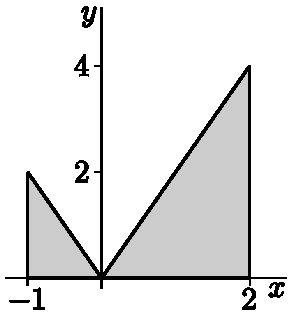
\includegraphics{OEM105_13A_1e}}
\end{align*}


\end{solution}
%%%%%%%%%%%%%%%%%%%

\begin{Mquestion}
Evaluate the following integral by interpreting it as a signed area, and using geometry:
\[\int_{-3}^5 |t-1| \,\dee{t}\]
\end{Mquestion}
\begin{hint}
Draw a picture. Remember $|x| = \left\{\begin{array}{rc}x&x\ge 0\\-x&x<0\end{array}\right.$\ .
\end{hint}
\begin{answer}
16
\end{answer}
\begin{solution}
The area we want is two triangles, both above the $x$-axis. Each triangle has base $4$ and height $4$, so the total area is $2\cdot\left(\dfrac{4\cdot 4}{2}\right)=16$.
\begin{center}
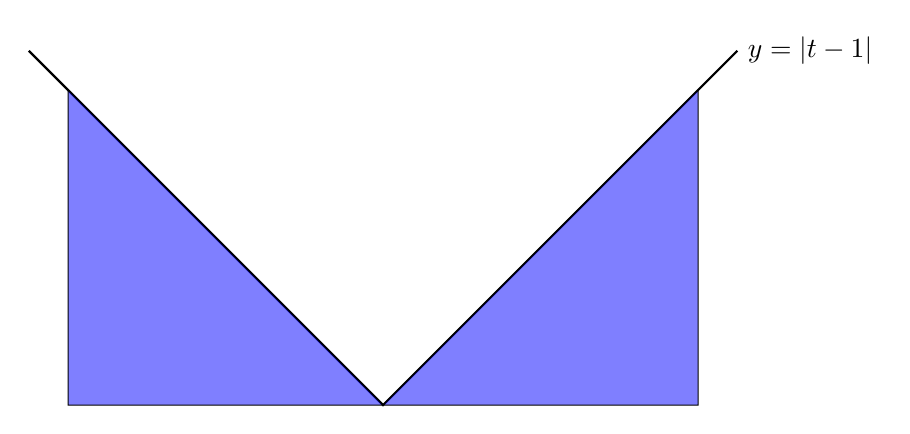
\begin{tikzpicture}
\YEaaxis{5}{6}{1}{5}
\draw[thick] (-3.5,4.5)--(1,0)--(5.5,4.5) node[right]{$y=|t-1|$};
\draw[fill=blue, fill opacity=0.5] (-3,0)--(-3,4)--(1,0)--(5,4)--(5,0)--cycle;
\YExcoord{5}{5}
\YExcoord{1}{1}
\YExcoord{-3}{-3}
\YEycoord{4}{4}
\end{tikzpicture}
\end{center}
If you had a hard time sketching the function, recall that the absolute value of a number leaves it unchanged if it is positive or zero, and flips the sign if it is negative. So, when $t-1 \ge 0$ (that is, when $t \ge 1$), our function is simply $f(t)=|t-1|=t-1$. On the other hand, when $t=1$ is negative (that is, when $t<1$), the absolute value changes the sign, so $f(t) = |t-1|=-(t-1)=-t+1$.
\end{solution}

\begin{question}\label{1.1trapezoidarea}
Evaluate the following integral by interpreting it as a signed area, and using geometry:
\[\int_a^b x \,\dee{x}\]
where $0 \leq a \leq b$.
\end{question}
\begin{hint}
Draw a picture: the area we want is a trapezoid. If you don't remember a formula for the area of a trapezoid, think of it as the difference of two triangles.
\end{hint}
\begin{answer}
$\dfrac{b^2-a^2}{2}$
\end{answer}
\begin{solution}
The area we want is a trapezoid with base $(b-a)$ and heights $a$ and $b$, so its area is $\dfrac{(b-a)(b+a)}{2}=\dfrac{b^2-a^2}{2}$.
\begin{center}
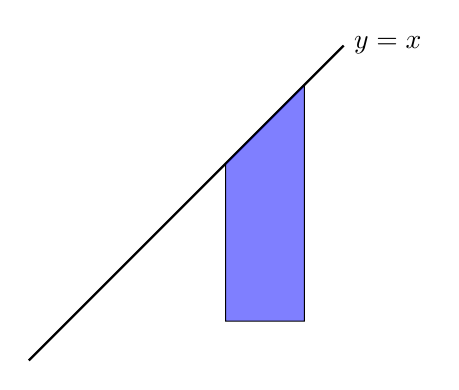
\begin{tikzpicture}
\YEaaxis{1}{4}{1}{4}
\draw[thick] (-.5,-.5)--(3.5,3.5) node[right]{$y=x$};
\draw[fill=blue, fill opacity=0.5] (2,0)--(2,2)--(3,3)--(3,0)--cycle;
\YExcoord{3}{b}
\YEycoord{3}{b}
\YExcoord{2}{a}
\YEycoord{2}{a}
\end{tikzpicture}
\end{center}
Instead of using a formula for the area of a trapezoid, you can find the blue area as the area of a triangle with base and height $b$, minus the area of a triangle with base and height $a$.
\end{solution}

\begin{question}
Evaluate the following integral by interpreting it as a signed area, and using geometry:
\[\int_a^b x\, \dee{x}\]
where $a \leq b \leq 0$.
\end{question}
\begin{hint}
You can draw a very similar picture to Question~\ref{1.1trapezoidarea}, but remember the areas are negative.
\end{hint}
\begin{answer}
$\dfrac{b^2-a^2}{2}$
\end{answer}
\begin{solution}
The area is negative. The shape is a trapezoid with base length $(b - a)$ and heights
        $0-a=-a$ and $0-b=-b$ (note: those are nonnegative numbers), so its area is $\dfrac{(b-a)(-b-a)}{2}=\dfrac{-b^2+a^2}{2}$. Since the shape is below the $x$-axis, we change its sign. Thus, the integral evaluates to\ $\dfrac{b^2-a^2}{2}$.
\begin{center}
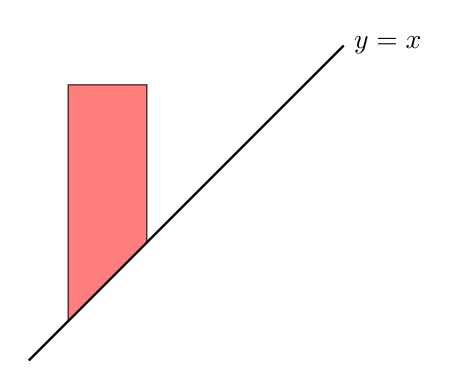
\begin{tikzpicture}
\YEaaxis{4}{1}{4}{1}
\draw[thick] (-3.5,-3.5)--(.5,.5) node[right]{$y=x$};
\draw[fill=red, fill opacity=0.5] (-2,0)--(-2,-2)--(-3,-3)--(-3,0)--cycle;
\YEnxcoord{-3}{a}
\YEnycoord{-3}{a}
\YEnxcoord{-2}{b}
\YEnycoord{-2}{b}
\end{tikzpicture}
\end{center}

The signs can be a little hard to keep track of. The base of our trapezoid is $|a-b|$;  since $b>a$, this is $b-a$. The heights of the trapezoid are  $|a|$ and $|b|$; since these are both negative, $|a|=-a$ and $|b|=-b$.

We note that this is the same result as in Question~\ref{1.1trapezoidarea}.
\end{solution}


\begin{Mquestion}
Evaluate the following integral by interpreting it as a signed area, and using geometry:
\[\int_0^4 \sqrt{16-x^2} \ \dee{x}\]
\end{Mquestion}
\begin{hint}
If $y=\sqrt{16-x^2}$, then $y$ is nonnegative, and $y^2+x^2=16$.
\end{hint}
\begin{answer}
$4\pi$
\end{answer}
\begin{solution}
If $y=\sqrt{16-x^2}$, then $y$ is nonnegative, and $y^2+x^2=16$. So, the graph $y=\sqrt{16-x^2}$ is the upper half of a circle of radius 4. Since $x$ only runs from 0 to 4, we have a quarter of a circle of radius 4. Then the area under the curve is $\dfrac{1}{4}\left[\pi\cdot 4^2\right]=4\pi$.
\begin{center}
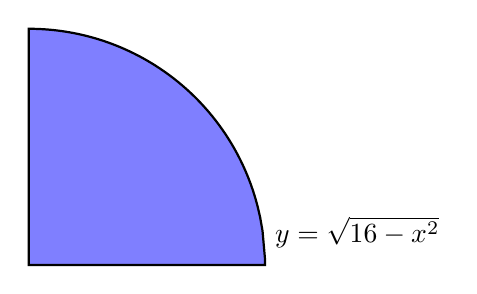
\begin{tikzpicture}
\YEaaxis{1}{6}{1}{4}
\draw[thick, fill=blue, fill opacity=0.5] plot[domain=0:3, samples=100] (\x,{sqrt(9-\x*\x)}) node[above right, opacity=1]{$y=\sqrt{16-x^2}$}--(3,0)--(0,0)--cycle;
\end{tikzpicture}
\end{center}
\end{solution}



\begin{Mquestion}[2016Q1]\label{1.1defintgeomb}
Use elementary geometry to calculate $\displaystyle \int_0^3 f(x)\,\,\dee{x}$, where
\begin{align*}
  f(x) = \begin{cases}
  x, & \text{if } x \le 1,\\
  1, & \text{if } x > 1.
  \end{cases}
\end{align*}

\end{Mquestion}

\begin{hint}
Sketch the graph of $f(x)$.
\end{hint}

\begin{answer}
$\displaystyle\int_0^3 f(x)\,\,\dee{x} = 2.5$
\end{answer}

\begin{solution}
Here is a sketch the graph of $f(x)$.

\begin{center}
    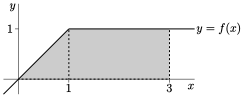
\includegraphics{OQ16_1}
\end{center}

\noindent
There is a linear increase from $x=0$ to $x=1$, followed by a constant. Using the interpretation of $\int_0^3 f(x)\,\,\dee{x}$ as the area between $y=f(x)$ and the
$x$--axis with $x$ between $0$ and $3$, we can break this area into:
\begin{itemize}
  \item $\int_0^1 f(x)\,\,\dee{x}$: a right-angled triangle of height $1$ and base $1$ and hence area $0.5$.
  \item $\int_1^3 f(x)\,\,\dee{x}$: a rectangle of height $1$ and base $2$ and hence
area $2$.
\end{itemize}
Summing up: $\int_0^3 f(x)\,\,\dee{x} = 2.5$.
\end{solution}
%%%%%%%%%%%%%%%%%%%




\begin{Mquestion}[2016Q1]\label{1.1cartime}
A car's gas pedal is applied at $t=0$ seconds and the car
accelerates continuously until $t=2$ seconds.
The car's speed at half-second intervals is given in the table
below.
Find the best possible \textbf{upper} estimate for the distance
that the car traveled during these two seconds.
\begin{center}
\renewcommand{\arraystretch}{1.3}
   \begin{tabular}{!{\vrule width 1pt}c!{\vrule width 1pt}c|c|c|c|c!{\vrule width 1pt}}
        \noalign{\hrule height 1pt}
        $t$ (s)  & $0$ & $0.5$ & $1.0$ & $1.5$ & $2$ \\    \hline
        $v$ (m/s) & 0 & 14 & 22 & 30 & 40 \\
      \noalign{\hrule height 1pt}
     \end{tabular}
\renewcommand{\arraystretch}{1.0}
\end{center}
\end{Mquestion}

\begin{hint}
At which time in the interval, for example, $0\le t\le 0.5$,  is the car moving
the fastest?
\end{hint}

\begin{answer}
53 m
\end{answer}

\begin{solution}
The car's speed increases with time. So its highest speed on any
time interval occurs at the right hand end of the interval and
the best possible upper estimate for the distance traveled is
given by the \emph{right} Riemann sum with $\Delta x =0.5$, which
is
\begin{equation*}
\big[v(0.5)+v(1.0)+v(1.5)+v(2.0)\big]\times 0.5
=\big[14+22+30+40\big]\times 0.5= 53\text{ m}
\end{equation*}
\end{solution}


\begin{Mquestion} True or false: the answer you gave for Question~\ref{1.1cartime} is definitely greater than or equal
to the distance the car travelled during the two seconds in question.
\end{Mquestion}
\begin{hint}
What are the possible speeds the car could have reached at time $t=0.25$?
\end{hint}
\begin{answer}
true
\end{answer}
\begin{solution}
There is a key detail in the statement of Question~\ref{1.1cartime}: namely, that the car is continuously accelerating. So, although we don't know exactly what's going on in between our brief snippets of information, we know that the car is not going any faster during an interval than at the end of that interval. Therefore, the car certainly travelled no farther than our estimation.

We ask this question in order to point out an important detail. If we did not have the information that the car was continuously accelerating, we would not be able to give a certain upper bound on its distance travelled. It would be possible that, when the car is not being observed (for example, when $t=0.25$), it is going much faster than when it is being observed.
\end{solution}



\begin{question}\label{1.1airtime}
An airplane's speed at one-hour intervals is given in the table below.
Approximate the distance travelled by the airplane from noon to 4pm using a midpoint Riemann sum.
\begin{center}
\renewcommand{\arraystretch}{1.3}
   \begin{tabular}{!{\vrule width 1pt}c!{\vrule width 1pt}c|c|c|c|c!{\vrule width 1pt}}
        \noalign{\hrule height 1pt}
        time  & 12:00 pm & 1:00 pm & 2:00 pm & 3:00 pm & 4:00 pm   \\
         \hline
        speed (km/hr) & 800 & 700 & 850 &900 & 750 \\
      \noalign{\hrule height 1pt}
     \end{tabular}
\renewcommand{\arraystretch}{1.0}
\end{center}

\end{question}
\begin{hint}
You need to know the speed of the plane at the midpoints of your intervals, so (for example) noon to 1pm \emph{is not} one of your intervals.
\end{hint}
\begin{answer}
3200 km
\end{answer}
\begin{solution}
First, note that the distance travelled by the plane is equal to the area under the graph of its speed.

We need to know the speed of the plane at the midpoints of our intervals. So (for example) noon to 1pm \emph{is not} one of your intervals--we don't know the speed at 12:30. (A common idea is to average the two end values, 700 and 800. This is a fine approximation, but it is not a Riemann sum.) So, we use the two intervals 12:00 to 2:00, and 2:00 to 4:00. Then our intervals have length 2 hours, and at the midpoints of the intervals the speed of the plane is 700 kph and 900 kph, respectively. So, our midpoint Riemann sum gives us:
\[700(2)+900(2) = 3200\]
an approximation of 3200 km travelled by the plane from noon to 4:00 pm.

Remark: if we had been asked to approximate the distance travelled from 11:30 am to 4:30 pm, then we could have used the midpoint rule with five intervals and made use of every entry in the data table. With the question as stated, however, we ignore three out of five entries in the table because they are not the midpoints of our intervals.
\end{solution}


%%%%%%%%%%%%%%%%%%
\subsection*{\Application}
%%%%%%%%%%%%%%%%%%

\begin{Mquestion}[2016Q1]
\noindent (a)
Express
\begin{equation*}
\lim_{n\rightarrow\infty}
     \sum_{i=1}^n\frac{2}{n}\sqrt{4-\left(-2+\frac{2i}{n}\right)^2}
\end{equation*}
as a definite integal.

\noindent (b)
Evaluate the integral of part (a).
\end{Mquestion}

\begin{hint}
Sure looks like a Riemann sum.
\end{hint}

\begin{answer}
(a) There are many possible answers. Two are
        $\int_{-2}^0 \sqrt{4-x^2}\,\,\dee{x}$ and
        $\int_0^2 \sqrt{4-(-2+x)^2}\,\,\dee{x}$.
\noindent
(b) $\pi$
\end{answer}

\begin{solution}
\begin{description}
\item[Solution \#1:]
Set $x_i^*=-2+\frac{2i}{n}$. Then $a=x_0=-2$
and $b=x_n=0$ and $\Delta x=\frac{2}{n}$. So
\begin{align*}
\lim_{n\rightarrow\infty}
     \sum_{i=1}^n\frac{2}{n}\sqrt{4-\left(-2+\frac{2i}{n}\right)^2}
&= \lim_{n\rightarrow\infty}
     \sum_{i=1}^n f(x_i^*)\Delta x\qquad
   \text{ with $f(x) = \sqrt{4-x^2}$ and $\Delta x = \frac{2}{n}$ } \\
&=\int_{-2}^0 \sqrt{4-x^2}\,\,\dee{x}
\end{align*}

For the integral $\int_{-2}^0 \sqrt{4-x^2}\,\,\dee{x}$,
$y=\sqrt{4-x^2}$ is equivalent to $x^2+y^2=4$,
$y\ge 0$. So the integral represents the area between the upper
half of the circle $x^2+y^2=4$ (which has radius $2$)
and the $x$-axis with $-2\le x\le 0$, which is a quarter circle with area
$\frac{1}{4}\cdot \pi\, 2^2 = \pi$.

\begin{center}
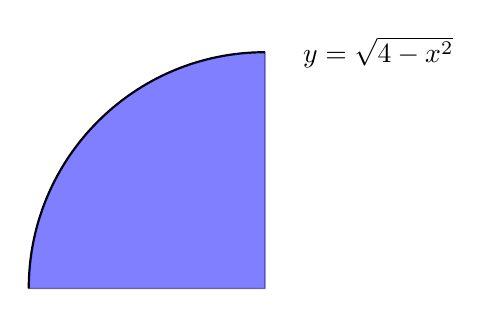
\begin{tikzpicture}
\YEaaxis{4}{1}{1}{3.5}
\draw[thick] (-3,0) arc (180:90:3cm) node[right]{\quad $y=\sqrt{4-x^2}$};
\draw[fill=blue, opacity=0.5] (-3,0) arc (180:90:3cm)--(0,0)--cycle;
\YExcoord{-3}{-{2}}
\end{tikzpicture}
\end{center}

\item[Solution \#2:]
Set $x_i^*=\frac{2i}{n}$. Then $a=x_0=0$
and $b=x_n=2$ and $\Delta x=\frac{2}{n}$. So
\begin{align*}
\lim_{n\rightarrow\infty}
     \sum_{i=1}^n\frac{2}{n}\sqrt{4-\left(-2+\frac{2i}{n}\right)^2}
&= \lim_{n\rightarrow\infty}
     \sum_{i=1}^n f(x_i^*)\Delta x\quad
   \text{ with $f(x) = \sqrt{4-(-2+x)^2}$, $\Delta x = \frac{2}{n}$ } \\
&=\int_0^2 \sqrt{4-(-2+x)^2}\,\,\dee{x}
\end{align*}

For the integral $\int_{0}^2  \sqrt{4-(-2+x)^2}\,\,\dee{x}$\ ,
$y=\sqrt{4-(x-2)^2}$ is equivalent to $(x-2)^2+y^2=4$,
$y\ge 0$. So the integral represents the area between the upper
half of the circle $(x-2)^2+y^2=4$ (which is centered at $(2,0)$ and has radius $2$)
and the $x$-axis with $0\le x\le 2$, which is a quarter circle with area
$\frac{1}{4}\cdot \pi\, 2^2 = \pi$.

\begin{center}
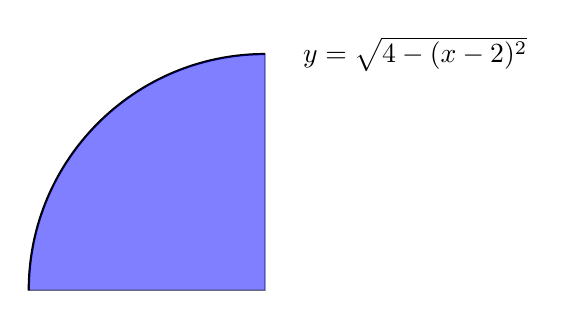
\begin{tikzpicture}
\YEaaxis{1}{4}{1}{3.5}
\draw[thick] (0,0) arc (180:90:3cm) node[right]{\quad $y=\sqrt{4-(x-2)^2}$};
\draw[fill=blue, opacity=0.5] (0,0) arc (180:90:3cm)--(3,0)--cycle;
\YExcoord{3}{{2}}
\end{tikzpicture}
\end{center}

\end{description}

\end{solution}
%%%%%%%%%%%%%%%%%%%%%%%%%%%%%%%%%%%%%%%

\begin{question}[2016Q1]
Consider the integral:
\begin{align*}
   \int_0^3 (7 + x^3) \,\,\dee{x} . ~~~~~~~~~ (*)
\end{align*}
\begin{enumerate} [(a)]
\item
   Approximate this integral using the left Riemann sum with $n=3$ intervals.
\item
    Write down the expression for the right Riemann sum with $n$
intervals and calculate the sum. Now take the limit $n \to \infty$
in your expression for the Riemann sum, to evaluate the integral
($*$) exactly.
\end{enumerate}
You may use the identity
\begin{align*}
\sum_{i=1}^{n} i^3 = \frac{n^4 +2n^3 + n^2}{4}
\end{align*}
\end{question}

\begin{hint}
For part (b): don't panic! Just take it one step at a time.
The first step is to write down the Riemann sum.
The second step is to evaluate the sum, using the given identity.
The third step is to evaluate the limit $n\rightarrow\infty$.
\end{hint}

\begin{answer}
(a) $30$
\qquad (b) $41 \frac{1}{4}$
\end{answer}

\begin{solution} (a)
The left Riemann sum is defined as
\begin{align*}
  L_n = \sum_{i=1}^{n}  f(x_{i-1})\Delta x
    \qquad\text{with }x_i=a+i\De x
\end{align*}
We subdivide into $n=3$ intervals, so that $\Delta x = \frac{b-a}{n}
=\frac{3-0}{3}=1$, $x_0=0$, $x_1=1$ and $x_2=2$.
The function $f(x) = 7 + x^3$ has the values
$f(x_0) = 7+0^3=7$,
$f(x_1) = 7+1^3=8$, and
$f(x_2) = 7+2^3=15$, from which we evaluate
\begin{align*}
L_3 = \big[f(x_0)+f(x_1)+f(x_2)\big]\De x = \big[7+8+15\big]\times 1= 30
\end{align*}

\noindent (b)
We divide into $n$ intervals so that
$\Delta x = \frac{b-a}{n}=\frac{3}{n}$ and  $x_i = a+i\De x= \frac{3i}{n}$.
The right Riemann sum is therefore:
\begin{align*}
R_n = \sum_{i=1}^{n}  f(x_i)\Delta x
    =  \sum_{i=1}^{n} \left[ 7 + \frac{(3i)^3}{n^3} \right] \frac{3}{n}
    =  \sum_{i=1}^{n} \left[ \frac{21}{n} + \frac{81\,i^3}{n^4} \right]
\end{align*}
To calculate the sum:
\begin{align*}
  R_n &= \left( \frac{21}{n} \sum_{i=1}^{n} 1 \right)
        +  \left( \frac{81}{n^4} \sum_{i=1}^{n} i^3 \right)\\
   &=\left( \frac{21}{n}\times n \right)+\left(  \frac{81}{n^4} \times \frac{n^4 +2n^3 + n^2}{4} \right)\\
                 &= 21 + \frac{81}{4}(1 +2/n + 1/n^2)
\end{align*}
To evaluate the limit exactly, we take $n \to \infty$. The expressions involving $1/n$ vanish leaving:
\begin{align*}
\int_0^3 (7 + x^3) \,\,\dee{x} = \lim_{n \to \infty} R_n = 21 + \frac{81}{4} = 41 \frac{1}{4}
\end{align*}

\end{solution}
%%%%%%%%%%%%%%%%%%%



\begin{question}[2013A]
Using a limit of right--endpoint Riemann
sums, evaluate $\displaystyle\int_2^4 x^2\ \,\dee{x}$. \\[5pt]
You may use the formulas
$\sum\limits_{i=1}^n i = \frac{n(n + 1)}{2}$ and
$\sum\limits_{i=1}^n i^2 = \frac{n(n + 1)(2n + 1)}{6}$.
\end{question}

\begin{hint}
The first step is to write down the Riemann sum.
The second step is to evaluate the sum, using the given formulas.
The third step is to evaluate the limit as $n\rightarrow\infty$.
\end{hint}

\begin{answer}
$\dfrac{56}{3}$
\end{answer}

\begin{solution}
In general, the right--endpoint Riemann sum
approximation to the integral $\int_a^b f(x)\,\,\dee{x}$ using $n$ rectangles is
\begin{align*}
\sum_{i=1}^n f(a+i\De x) \De x
\end{align*}
where $\De x=\frac{b-a}{n}$. In this problem, $a=2$, $b=4$, and $f(x)=x^2$,
so that $\De x=\frac{2}{n}$ and the  right--endpoint Riemann
sum approximation becomes
\begin{align*}
\sum_{i=1}^n f\Big(2+\frac{2i}{n}\Big) \frac{2}{n}&=
\sum_{i=1}^n \Big(2+\frac{2i}{n}\Big)^2 \frac{2}{n}\\
&=\sum_{i=1}^n \left(4+\frac{8i}{n}+\frac{4i^2}{n^2}\right)\frac{2}{n}
\\&=\sum_{i=1}^n \left(\frac{8}{n}+\frac{16i}{n^2}+\frac{8i^2}{n^3}\right)
\\&=\sum_{i=1}^n \frac{8}{n}+\sum_{i=1}^n \frac{16i}{n^2}
  +\sum_{i=1}^n \frac{8i^2}{n^3} \cr
&=\frac{8}{n}\sum_{i=1}^n 1+\frac{16}{n^2}\sum_{i=1}^n i
  +\frac{8}{n^3}\sum_{i=1}^n i^2\cr
&=\frac{8}{n}n + \frac{16}{n^2}\cdot\frac{n(n+1)}{2}
  +\frac{8}{n^3}\cdot\frac{n(n + 1)(2n + 1)}{6} \cr
&=8 + 8\Big(1+\frac{1}{n}\Big)
  +\frac{4}{3}\Big(1+\frac{1}{n}\Big)\Big(2+\frac{1}{n}\Big) \cr
\end{align*}
So
\begin{align*}
\int_2^4 x^2\ \,\dee{x}=\lim_{n\rightarrow\infty}
                      \Big[8 + 8\Big(1+\frac{1}{n}\Big)
                            +\frac{4}{3}\Big(1+\frac{1}{n}\Big)
                             \big(2+\frac{1}{n}\Big)\Big]
=8+8+\frac{4}{3}\times 2
=\frac{56}{3}
\end{align*}
\end{solution}
%%%%%%%%%%%%%%%%%%%

\begin{question}[2016Q1]
Find $\displaystyle\int_0^2 (x^3+x)\,\,\dee{x}$ using the definition of the definite integral.
You may use the summation formulas $\sum\limits_{i=1}^{n}i^3 = \frac{n^4+2n^3+n^2}4$ and
$\sum\limits_{i=1}^{n} i = \frac{n^2+n}{2}$.
\end{question}

\begin{hint}
The first step is to write down the Riemann sum.
The second step is to evaluate the sum, using the given formulas.
The third step is to evaluate the limit $n\rightarrow\infty$.
\end{hint}

\begin{answer}
$6$
\end{answer}

\begin{solution}
We'll use right Riemann sums with $a=0$ and $b=2$. When there are $n$ rectangles,
$\Delta x = \frac{b-a}{n}=\frac{2}{n}$ and  $x_i = a+i\De x=2i/n$.  So
we need to evaluate
\begin{align*}
\lim_{n\to\infty} \sum_{i=1}^{n} f(x_i)\De x
&=\lim_{n\to\infty} \sum_{i=1}^{n} \left( (x_i)^3 + x_i\right) \De x\\
  &=\lim_{n\to\infty} \sum_{i=1}^{n} \left( \left(\frac{2i}{n}\right)^3 + \frac{2i}{n}\right)
             \frac{2}{n} \\
   & = \lim_{n\to\infty} \frac{2}{n} \sum_{i=1}^{n} \left(\frac{8i^3}{n^3} + \frac{2i}{n}\right) \\
&= \lim_{n\to\infty} \left( \frac{16}{n^4} \sum_{i=1}^{n} i^3 + \frac{4}{n^2} \sum_{i=1}^{n} i \right) \\
   & = \lim_{n\to\infty} \left( \frac{16(n^4+2n^3+n^2)}{n^4 \cdot 4} + \frac{4(n^2+n)}{n^2 \cdot 2} \right) \\
&= \lim_{n\to\infty} \left( \frac{16}{4}\left(1+\frac{2}{n} + \frac1{n^2} \right) + \frac{4}{2}\left(1+\frac{1}{n}\right)\right) \\
& = \frac{16}{4} + \frac{4}{2} = 6.
\end{align*}
\end{solution}

%%%%%%%%%%%%%%%%%%%

\begin{Mquestion}[2014D]
Using a limit of right--endpoint Riemann sums, evaluate
$\displaystyle\int_1^4 (2x-1)\,\,\dee{x}$.
Do not use  anti-differentiation, except to check your answer.\footnote{You'll learn about this method starting in Section~\eref{CLP101}{sec fundamental} of the CLP-2 text.
You can also check this answer using geometry.}
You may use the formula $\sum\limits_{i=1}^{n} i = \frac{n(n+1)}{2}$.
\end{Mquestion}

\begin{hint}
You've probably seen this hint before. It is worth repeating.
Don't panic! Just take it one step at a time.
The first step is to write down the Riemann sum.
The second step is to evaluate the sum, using the given formula.
The third step is to evaluate the limit $n\rightarrow\infty$.
\end{hint}

\begin{answer}
$12$
\end{answer}

\begin{solution}
We'll use right Riemann sums with $a=1$, $b=4$ and $f(x) =2x-1$.
When there are $n$ rectangles, $\Delta x = \frac{b-a}{n}=\frac{3}{n}$ and
$x_i = a+i\De x=1 + 3i/n$.  So we need to evaluate
\begin{align*}
\lim_{n\to\infty} \sum_{i=1}^{n} f(x_i) \De x
& = \lim_{n\to\infty} \sum_{i=1}^{n} \left( 2x_i - 1\right) \De x\\
 & =\lim_{n\to\infty} \sum_{i=1}^{n} \left(2+ \frac{6i}{n}-1\right)\frac{3}{n} \\
& = \lim_{n\to\infty} \frac{3}{n} \sum_{i=1}^{n} \left(\frac{6i}{n}+1\right) \\
&= \lim_{n\to\infty} \left( \frac{18}{n^2} \sum_{i=1}^{n} i
                            + \frac{3}{n} \sum_{i=1}^{n} 1 \right) \\
& = \lim_{n\to\infty} \left(\frac{18\cdot n(n+1)}{n^2\cdot 2}
                              + \frac{3}{n}n\right)\\
&= \lim_{n\to\infty} \left(9\left(1+\frac{1}{n}\right) + 3\right) \\
& = 9 + 3 = 12.
\end{align*}
\end{solution}


\begin{question}
Give a function $f(x)$ that has the following expression as a right Riemann sum when $n=10$, $\Delta(x)=10$ and $a=-5$:
\[\sum_{i=1}^{10} 3(7+2i)^2\sin(4i)\,.\]
\end{question}
\begin{hint}
Using the definition of a right Riemann sum,  we can come up with an expression for
$f(-5+10i)$. In order to find $f(x)$, set $x=-5+10i$.
\end{hint}
\begin{answer}
$f(x)=\dfrac{3}{10}\left(\dfrac{x}{5}+8\right)^2\sin\left(\dfrac{2x}{5}+2\right)$
\end{answer}
\begin{solution}
Using the definition of a right Riemann sum,
\begin{align*}
\displaystyle\sum_{i=1}^{10} 3(7+2i)^2\sin(4i) &= \displaystyle\sum_{i=1}^{10} \Delta x f(a+i\Delta x)
\intertext{Since $\Delta x = 10$ and $a=-5$,}
\displaystyle\sum_{i=1}^{10} 3(7+2i)^2\sin(4i) &= \displaystyle\sum_{i=1}^{10} 10 f(-5+10i)
\intertext{Dividing both expressions by 10,}
\displaystyle\sum_{i=1}^{10} \frac{3}{10}(7+2i)^2\sin(4i) &= \displaystyle\sum_{i=1}^{10}  f(-5+10i)
\intertext{So, we have an expression for $f(-5+10i)$:}
f(-5+10i) &= \frac{3}{10}(7+2i)^2\sin(4i)
\intertext{In order to find $f(x)$, let $x=-5+10i$. Then $i=\frac{x}{10}+\frac{1}{2}$.}
f(x) &= \frac{3}{10}\left(7+2\left(\frac{x}{10}+\frac{1}{2}\right)\right)^2\sin\left(4\left(\frac{x}{10}+\frac{1}{2}\right)\right)\\
&=\frac{3}{10}\left(\frac{x}{5}+8\right)^2\sin\left(\frac{2x}{5}+2\right)\ .
\end{align*}
\end{solution}


\begin{question}\label{1.1_2x}
Using the method of Example~\eref{CLP101}{eg:INTexpareaB} in the CLP-2 text, evaluate
\[\int_0^1 2^x \ \dee{x}\]
\end{question}
\begin{hint}
Recall that for a positive constant $a$, $\diff{}{x}\left\{a^x\right\} = a^x \log a$, where $\log a$ is the natural logarithm (base $e$) of $a$.
\end{hint}
\begin{answer}
$\dfrac{1}{\log 2}$
\end{answer}
\begin{solution}
As in the text, we'll set up a Riemann sum for the given integral. Right Riemann sums have the simplest form, so we use a right Riemann sum, but we could equally well use left or midpoint.
\begin{align*}
\int_0^1 2^x\dee{x}&=\lim_{n \to \infty}\sum_{i=1}^n \Delta x f({a+i\Delta x})\\
&=\lim_{n \to \infty}\sum_{i=1}^n \frac{1}{n} f\left(\frac{i}{n}\right)\\
&=\lim_{n \to \infty}\sum_{i=1}^n  \frac{1}{n}\cdot 2^{i/n}\\
&=\lim_{n \to \infty}\frac{1}{n}\left(2^{1/n}+2^{2/n}+2^{3/n}+\cdots + 2^{n/n}\right)\\
&=\lim_{n \to \infty}\frac{2^{1/n}}{n}\left(1+2^{1/n}+2^{2/n}+\cdots + 2^{\frac{n-1}{n}}\right)\\
&=\lim_{n \to \infty}\frac{2^{1/n}}{n}\left(1+2^{1/n}+\left(2^{1/n}\right)^2+\cdots + \left(2^{1/n}\right)^{n-1}\right)
\intertext{The sum in parenthesis has the form of a geometric sum, with $r=2^{1/n}$:}
&=\lim_{n \to \infty}\frac{2^{1/n}}{n}\left(
\frac{\left(2^{1/n}\right)^n-1}{2^{1/n}-1}
\right)\\
&=\lim_{n \to \infty}\frac{2^{1/n}}{n}\left(
\frac{2-1}{2^{1/n}-1}
\right)\\
&=\lim_{n \to \infty}
\frac{2^{1/n}}{n(2^{1/n}-1)}
\intertext{Note as $n \to \infty$, $1/n \to 0$, so the numerator has limit 1, while the denominator has indeterminate form $\infty\cdot 0$. So, we'll do a little algebra to get this into a l'H\^opital-style indeterminate form:}
&=\lim_{n \to \infty}
\frac{\frac{1}{n}\cdot2^{1/n}}{2^{1/n}-1}
\\&=\lim_{n \to \infty}
\underbrace{\frac{\frac{1}{n}}{1-2^{-1/n}}}_{\atp{\mathrm{num}\to 0}{\mathrm{den}\to 0}}
\intertext{Now we can use l'H\^opital's rule. Recall $\diff{}{x}\left\{2^x\right\}=2^x\log x$, where $\log x$ is the natural logarithm of $x$, also sometimes written $\ln x$. We'll need to use the chain rule when we differentiate the denominator.}
&=\lim_{n \to \infty}
\frac{\frac{-1}{n^2}}{-2^{-1/n}\log 2 \cdot \frac{1}{n^2}}
\\&=\lim_{n \to \infty}
\frac{2^{1/n}}{\log 2}\\
&=\frac{1}{\log 2}
\end{align*}
Using a calculator, we see this is about 1.44 square units.
\end{solution}

\begin{question}
\begin{enumerate}[(a)]
\item Using the method of Example~\eref{CLP101}{eg:INTexpareaB} in the CLP-2 text, evaluate
\[\int_a^b 10^x \ \dee{x}\]
\item
\end{enumerate} Using your answer from above, make a guess for
\[\int_a^b c^x \ \dee{x}\]
where $c$ is a positive constant. Does this agree with Question~\ref{1.1_2x}?
\end{question}
\begin{hint}
Part (a) follows  the same pattern as Question~\ref{1.1_2x}--there's just a little more algebra involved, since our lower limit of integration is not 0.
\end{hint}
\begin{answer}
(a) $\dfrac{1}{\log 10}\left(10^b-10^a\right)$\\
(b) $\dfrac{1}{\log c}\left(c^b-c^a\right)$; yes, it agrees.
\end{answer}
\begin{solution}
As in the text, we'll set up a Riemann sum for the given integral. Right Riemann sums have the simplest form:
\begin{align*}
\int_a^b 10^x\dee{x}&=\lim_{n \to \infty}\sum_{i=1}^n \Delta x f({a+i\Delta x})\\
&=\lim_{n \to \infty}\sum_{i=1}^n \frac{b-a}{n} f\left(a+i\frac{b-a}{n}\right)\\
&=\lim_{n \to \infty}\sum_{i=1}^n  \frac{b-a}{n}\cdot 10^{a+i\frac{b-a}{n}}\\
&=\lim_{n \to \infty}\sum_{i=1}^n  \frac{b-a}{n}\cdot 10^a\cdot \left(10^{\frac{b-a}{n}}\right)^{i}\\
&=\lim_{n \to \infty} \frac{b-a}{n}\cdot 10^a\left(\left(10^{\frac{b-a}{n}}\right)^1+
\left(10^{\frac{b-a}{n}}\right)^2
+\left(10^{\frac{b-a}{n}}\right)^3
+\cdots + \left(10^{\frac{b-a}{n}}\right)^n
\right)\\
&=\lim_{n \to \infty} \frac{b-a}{n}
\cdot10^{a}\cdot10^{\frac{b-a}{n}}
\left(1+\left(10^{\frac{b-a}{n}}\right)+
\left(10^{\frac{b-a}{n}}\right)^2
+\cdots + \left(10^{\frac{b-a}{n}}\right)^{n-1}
\right)
\intertext{Now the sum in parentheses has the form of a geometric sum, with $r=10^{\frac{b-a}{n}}$:}
&=\lim_{n \to \infty}
\frac{b-a}{n}\cdot
10^{a}\cdot 10^{\frac{b-a}{n}}\left(
\frac{\left(10^{\frac{b-a}{n}}\right)^n-1}{10^{\frac{b-a}{n}}-1}
\right)\\
&=\lim_{n \to \infty}
\frac{\textcolor{blue}{b-a}}{n}\cdot
\textcolor{red}{10^{a}}\cdot 10^{\frac{b-a}{n}}\left(
\frac{\textcolor{purple}{10^{b-a}-1}}{10^{\frac{b-a}{n}}-1}
\right)
\intertext{The coloured parts do not depend on $n$, so for simplicity we can move them outside the limit.}
&=\textcolor{blue}{(b-a)}\cdot\textcolor{red}{10^a}\left(\textcolor{purple}{10^{b-a}-1}\right)\lim_{n \to \infty}
\frac{1}{n}\cdot
\left(
\frac{ 10^{\frac{b-a}{n}} }{10^{\frac{b-a}{n}}-1}
\right)
\\&={(b-a)}\cdot\left({10^{b}-10^a}\right)\lim_{n \to \infty}
\underbrace{\left(
\frac{ 1/n}{1-10^{-\frac{b-a}{n}}}
\right)}_{\atp{\mathrm{num}\to 0}{\mathrm{den}\to 0}}
\intertext{Now we can use l'H\^opital's rule. Recall $\diff{}{x}\left\{10^x\right\}=10^x\log x$, where $\log x$ is the natural logarithm of $x$, also sometimes written $\ln x$. For the denominator, we will have to use the chain rule.}
&={(b-a)}\cdot\left({10^{b}-10^a}\right)\lim_{n \to \infty}
\left(
\frac{ -1/n^2}{-10^{-\frac{b-a}{n}}\cdot \log 10 \cdot \frac{b-a}{n^2}}
\right)\\
&={(b-a)}\cdot\left({10^{b}-10^a}\right)\lim_{n \to \infty}
\left(
\frac{ 1}{10^{-\frac{b-a}{n}}\cdot \log 10 \cdot (b-a)}
\right)\\
&={(b-a)}\cdot\left({10^{b}-10^a}\right)
\left(
\frac{ 1}{ \log 10 \cdot (b-a)}
\right)\\
&=\frac{1}{\log 10}\left(10^b-10^a\right)
\end{align*}

For part (b), we can guess that if 10 were changed to $c$, our answer would be
\[\int_a^b c^x \ \dee{x}=\frac{1}{\log c}\left(c^b-c^a\right)\]
In Question~\ref{1.1_2x}, we had $a=0$, $b=1$, and $c=2$. In this case, the formula we guessed above gives
\[\int_0^1 2^x \ \dee{x}=\frac{1}{\log 2}\left(2^1-2^0\right)=\frac{1}{\log2}\]
This does indeed match the answer we calculated.

(In fact, we can directly show $\displaystyle\int_a^b c^x \ \dee{x}=\dfrac{1}{\log c}\left(c^b-c^a\right)$ using the method of this problem.)
\end{solution}


\begin{Mquestion}\label{1.1_awkwardcircle} Evaluate $\displaystyle\int_0^a \sqrt{1-x^2}\ \dee{x}$ using geometry, if $0
\leq a \leq 1$.
\end{Mquestion}
\begin{hint}
Your area can be divided into a section of a circle and a triangle. Then you can use geometry to find the area of each piece.
\end{hint}
\begin{answer}
$\frac{\pi}{4} -\frac{1}{2} \arccos(a) + \frac{1}{2}a\sqrt{1-a^2}$
\end{answer}
\begin{solution}
First, we note $y=\sqrt{1-x^2}$ is the upper half of a circle of radius 1, centred at the origin. We're taking the area under the curve from 0 to $a$, so the area in question is as shown in the picture below.

\begin{center}
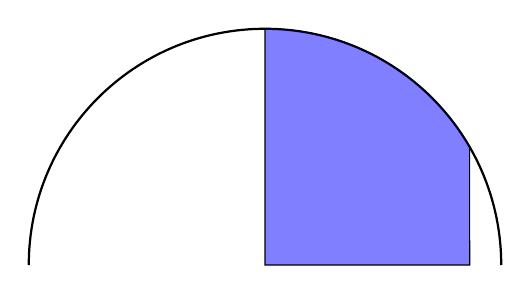
\begin{tikzpicture}
\YEaaxis{4}{4}{1}{4}
\YExcoord{-3}{-1}
\YExcoord{3}{1}
\YExcoord{2.6}{a}
\draw[thick] (-3,0) arc (180:0:3cm);
\draw[fill=blue, fill opacity=0.5] (0,0)--(0,3) arc(90:30:3cm)--(2.6,0)--cycle;
\end{tikzpicture}
\end{center}

In order to use geometry to find this area, we break it up into two pieces: a sector of a circle, and a triangle, shown below.

\begin{center}
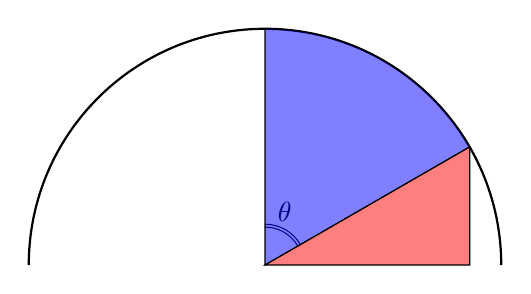
\begin{tikzpicture}
\YEaaxis{4}{4}{1}{4}
\YExcoord{-3}{-1}
\YExcoord{3}{1}
\YExcoord{2.6}{a}
\draw[thick] (-3,0) arc (180:0:3cm);
\draw[double](0,.5) arc (90:30:.5cm) node[midway, above]{$\theta$};
\draw[fill=blue, fill opacity=0.5] (0,0)--(0,3) arc(90:30:3cm)--cycle;
\draw[fill=red, fill opacity=0.5] (0,0)--(2.6,0)--(2.6,1.5)--cycle;
\end{tikzpicture}
\end{center}
\begin{description}
\item[Area of sector:] The sector is a portion of a circle with radius 1, with inner angle $\theta$. So, its area is $\frac{\theta}{2\pi}\left(\mbox{area of circle}\right) = \frac{\theta}{2\pi}\left(\pi\right) = \frac{\theta}{2}$.

Our job now is to find $\theta$ in terms of $a$. Note $\frac{\pi}{2}-\theta$ is the inner angle of the red triangle, which lies in the unit circle. So, $\cos\left(\frac{\pi}{2}-\theta\right)=a$. Then $\frac{\pi}{2}-\theta= \arccos(a)$, and so $\theta = \frac{\pi}{2} - \arccos(a)$.

Then the area of the sector is $\frac{\pi}{4} - \frac{1}{2}\arccos(a)$ square units.
\item[Area of triangle:] The triangle has base $a$. Its height is the $y$-value of the function when $x=a$, so its height is $\sqrt{1-a^2}$. Then the area of the triangle is $\frac{1}{2}a\sqrt{1-a^2}$.
\end{description}
We conclude $\displaystyle\int_0^a \sqrt{1-x^2}\ \dee{x} = \frac{\pi}{4} -\frac{1}{2} \arccos(a) + \frac{1}{2}a\sqrt{1-a^2}$.
\end{solution}



\begin{question}\label{1.1errornotaylor}
Suppose $f(x)$ is a positive, decreasing function from $x=a$ to $x=b$. You give an upper and lower bound on the area under the curve $y=f(x)$ using $n$ rectangles and a left and right Riemann sum, respectively, as in the picture below.

\begin{center}
\begin{tikzpicture}[scale=0.8]
\YEaaxis{1}{7.5}{1}{5}
\draw[red, pattern=crosshatch, pattern color=red] (1,0)--(1,4.25)-|(2,2.9)-|(3,1.85)-|(4,1.1)-|(5,0.65)-|(6,0.5)-|(6,0)--cycle;
\draw[thick] plot[domain=0.75:6.25, samples=100] (\x,{.15*(\x-6)*(\x-6)+.5}) node[right]{$y=f(x)$};
\draw[ fill=black, fill opacity=0.25] (1,0)--plot[domain=1:6, samples=100] (\x,{.15*(\x-6)*(\x-6)+.5}) --(6,0)--cycle;
\foreach \x in {1,...,6}{
\SUBTRACT{\x}{6}{\y}
\MULTIPLY{\y}{\y}{\z}
\MULTIPLY{\z}{0.15}{\w}
\ADD{\w}{0.5}{\c}
\draw[red, thick] (\x,0)--(\x,\c);}
\YExcoord{1}{a};
\YExcoord{6}{b};
\end{tikzpicture}
\hfill
\begin{tikzpicture}[scale=0.8]
\YEaaxis{1}{7.5}{1}{5}
\draw[red, pattern=crosshatch, pattern color=red] (1,0)--(1,2.9)-|(2,1.859)-|(3,1.1)-|(4,0.65)-|(5,0.5)-|(6,0)--cycle;
\draw[thick] plot[domain=0.75:6.25, samples=100] (\x,{.15*(\x-6)*(\x-6)+.5}) node[right]{$y=f(x)$};
\draw[fill=black, fill opacity=0.25] (1,0)--plot[domain=1:6, samples=100] (\x,{.15*(\x-6)*(\x-6)+.5}) --(6,0)--cycle;
\foreach \x in {2,...,6}{
\SUBTRACT{\x}{6}{\y}
\MULTIPLY{\y}{\y}{\z}
\MULTIPLY{\z}{0.15}{\w}
\ADD{\w}{0.5}{\c}
\draw[red, thick] (\x,0)--(\x,\c);}
\YExcoord{1}{a};
\YExcoord{6}{b};
\end{tikzpicture}
\end{center}
\begin{enumerate}[(a)]
\item\label{riemannerrorbounda} What is the difference between the lower bound and the upper bound? (That is, if we subtract the smaller estimate from the larger estimate, what do we get?) Give your answer in terms of $f$, $a$,  $b$, and $n$.
\item If you want to approximate the area under the curve to within 0.01 square units using this method, how many rectangles should you use? That is, what should $n$ be?
\end{enumerate}
\end{question}
\begin{hint}
\begin{enumerate}[(a)]
\item The difference between the upper and lower bounds is the area that is outside of the smaller rectangles but inside the larger rectangles.  Drawing both sets of rectangles on one picture might make things clearer. Look for an easy way to compute the area you want.
\item Use your answer from Part~(\ref{riemannerrorbounda}). Your answer will depend on $f$, $a$, and $b$.
\end{enumerate}
\end{hint}
\begin{answer}
\begin{enumerate}[(a)]
\item
$\left[f(b)-f(a)\right]\cdot\dfrac{b-a}{n}$
\item Choose $n$ to be an integer that is greater than or equal to $100\left[f(b)-f(a)\right](b-a)$.
\end{enumerate}
\end{answer}
\begin{solution}
\begin{enumerate}[(a)]
\item
The difference between our upper and lower bounds is the difference in areas between the larger set of rectangles and the smaller set of rectangles. Drawing them on a single picture makes this a little clearer.
\begin{center}
\begin{tikzpicture}
\YEaaxis{1}{7.5}{1}{5}
\draw[red, pattern=north east lines, pattern color=red] (1,0)--(1,4.25)-|(2,2.9)-|(3,1.85)-|(4,1.1)-|(5,0.65)-|(6,0.5)-|(6,0)--cycle;
\draw[purple, pattern=north west lines, pattern color=purple] (1,0)--(1,2.9)-|(2,1.859)-|(3,1.1)-|(4,0.65)-|(5,0.5)-|(6,0)--cycle;
\draw[thick] plot[domain=0.75:6.25, samples=100] (\x,{.15*(\x-6)*(\x-6)+.5}) node[right]{$y=f(x)$};
\foreach \x in {2,...,6}{
\SUBTRACT{\x}{6}{\y}
\MULTIPLY{\y}{\y}{\z}
\MULTIPLY{\z}{0.15}{\w}
\ADD{\w}{0.5}{\c}
\draw[purple, thick] (\x,0)--(\x,\c);}
\YExcoord{1}{a};
\YExcoord{6}{b};
\end{tikzpicture}
\end{center}

Each of the rectangles has width $\frac{b-a}{n}$, since we took a segment of the $x$-axis with length $b-a$ and chopped it into $n$ pieces. We could calculate the height of each rectangle, but it would be a little complicated, since it differs for each of them. An easier method is to notice that the area we want to calculate can be imagined as a single rectangle:

\begin{center}
\begin{tikzpicture}
\YEaaxis{1}{7.5}{1}{5}
\draw[thick] plot[domain=0.75:6.25, samples=100] (\x,{.15*(\x-6)*(\x-6)+.5}) node[right]{$y=f(x)$};
\YExcoord{1}{a};
\YExcoord{6}{b};
\draw[red, pattern=north east lines, pattern color=red] (1,4.25) rectangle (2,2.9) rectangle (3,1.85) rectangle (4,1.1) rectangle (5,0.65) rectangle (6,0.5);
\YEycoord{4.25}{f(a)}
\YEycoord{.5}{f(b)}
\draw[dotted] (0.2,4.25)--(1,4.25) (0.2,0.5)--(6,.5);
\draw[ultra thick, red, ->] (7,3) -- (9,3);

\draw[red, pattern=north east lines, pattern color=red] (11,4.25) rectangle (12,.5);
\foreach \y in {2.9,1.85,1.1,.65}{
	\draw[thick, red] (11,\y)--(12,\y);}
\end{tikzpicture}
\end{center}

The rectangle has base $\frac{b-a}{n}$. Its highest coordinate is $f(a)$, and its lowest is $f(b)$, so its height is $f(b)-f(a)$. Therefore, the difference in area between our lower bound and our upper bound is:
\[\left[f(b)-f(a)\right]\cdot\frac{b-a}{n}\]
\item We want to give a range with length at most 0.01, and guarantee that the area under the curve $y=f(x)$ is inside that range. In the previous part, we figured out that when we use $n$ rectangles, the length of our range is $\left[f(b)-f(a)\right]\cdot\frac{b-a}{n}$. So, all we have to do is set this to be less than or equal to 0.01, and solve for $n$:
\begin{align*}
\left[f(b)-f(a)\right]\cdot\frac{b-a}{n}&\leq 0.01 \\
100\left[f(b)-f(a)\right]\cdot(b-a)&\leq n
\end{align*}

We can choose $n$ to be an integer that is greater than or equal to $100\left[f(b)-f(a)\right]\cdot(b-a)$. Using that many rectangles, we find an upper and lower bound for the area under the curve. If we choose any number between our upper and lower bound as an approximation for the area under the curve, our error is no more than 0.01.
\end{enumerate}

Remark: this question depends on the fact that $f$ is decreasing and positive from $a$ to $b$. In general, bounding errors on approximations like this is not so straightforward.
\end{solution}


\begin{question}
Let $f(x)$ be a linear function,  let $a<b$ be integers, and let $n$ be a whole number. True or false: if we average the left and right Riemann sums for $\displaystyle\int_a^b f(x)\ \dee{x}$ using $n$ rectangles, we get the same value as the midpoint Riemann sum using $n$ rectangles.
\end{question}
\begin{hint}
Since $f(x)$ is linear, there exist real numbers $m$ and $c$ such that $f(x)=mx+c$. It's a little easier to first look at a single triangle from each sum, rather than the sums in their entirety.
\end{hint}
\begin{answer}
true (but note, for a non-linear function, it is possible that the midpoint Riemann sum is \emph{not} the average of the other two)
\end{answer}
\begin{solution}
Since $f(x)$ is linear, there exist real numbers $m$ and $c$ such that $f(x)=mx+c$. Now we can do some calculations. Suppose we have a rectangle in our Riemann sum that takes up the interval $[x,x+w]$.
\begin{itemize}
\color{blue} \item If we are using a left Riemann sum, our rectangle has height $f(x)=mx+c$.
Then it has area $w(mx+c)$. \color{red}
\item If we are using a right Riemann sum, our rectangle has height $f(x+w)=m(x+w)+c=mx+c+mw$. Then it has area $w(mx+c+mw)$.\color{black}
\item If we are using a midpoint Riemann sum, our rectangle has height $f(x+\frac{1}{2}w)=m(x+\frac{1}{2}w)+c=mx+c+\frac{1}{2}mw$.   Then it has area $w\left(mx+c+\frac{1}{2}w\right)$.
\end{itemize}
So, for each rectangle in our sums, the midpoint rectangle  has the same area as the average of the left and right rectangles:
\[w\left(mx+c+\frac{1}{2}mw\right) = \dfrac{\textcolor{blue}{w(mx+c)}+\textcolor{red}{w(mx+c+mw)}}{2}\]
It follows that the midpoint Riemann sum has a value equal to the average of the values of the left and right Riemann sums. To see this, let the rectangles in the midpoint Riemann sum have areas $M_1,M_2,\ldots,M_n$,
let the rectangles in the left Riemann sum have areas $\textcolor{blue}{L_1,L_2,\ldots,L_n}$, and
let the rectangles in the right Riemann sum have areas $\textcolor{red}{R_1,R_2,\ldots,R_n}$. Then the midpoint Riemann sum evaluates to $M_1+M_2+\cdots+M_n$, and:
\begin{align*}\dfrac{\textcolor{blue}{[L_1+L_2+\ldots+L_n]}+
\textcolor{red}{[R_1+R_2+\ldots+R_n]}
}{2} &=
\dfrac{\textcolor{blue}{L_1}+
\textcolor{red}{R_1}
}{2}+
\dfrac{\textcolor{blue}{L_2}+
\textcolor{red}{R_2}
}{2}+
\cdots
+
\dfrac{\textcolor{blue}{L_n}+
\textcolor{red}{R_n}
}{2} \\
&=M_1+M_2+\cdots+M_n\end{align*}
So, the statement is true.

(Note, however, it is false for many non-linear functions $f(x)$.)
\end{solution}
